% Created by tikzDevice version 0.7.0 on 2014-06-17 20:11:14
% !TEX encoding = UTF-8 Unicode
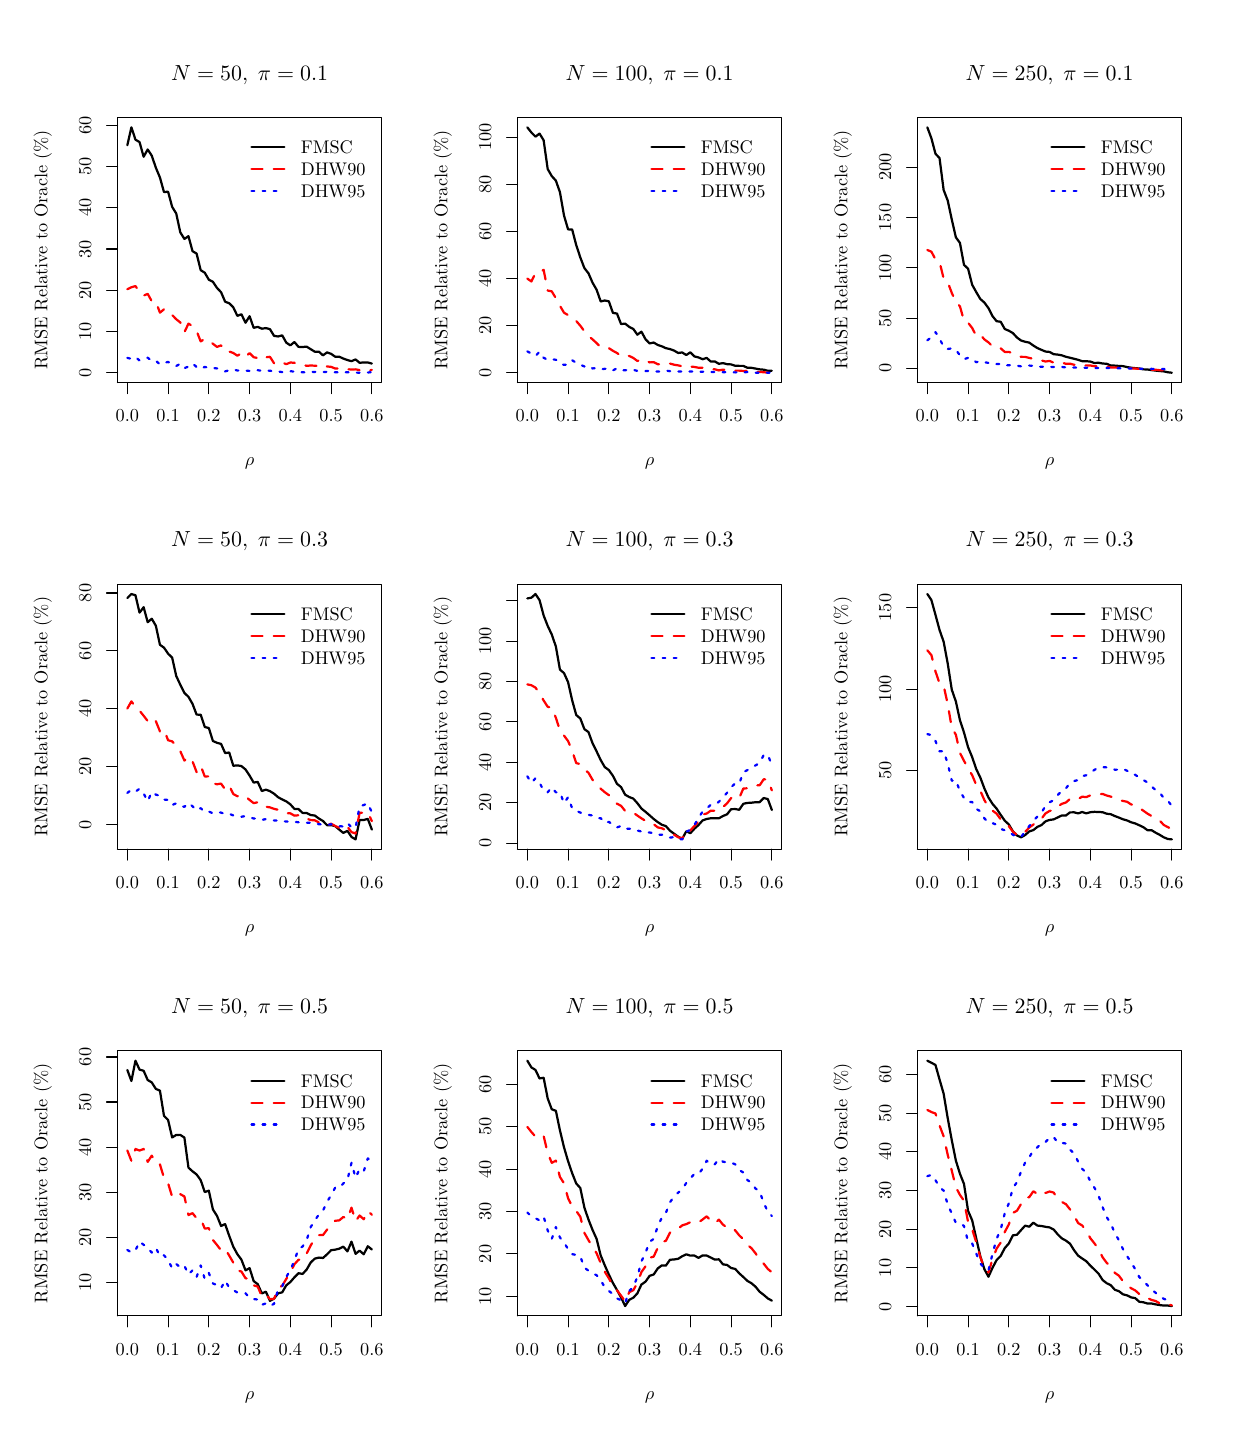
\begin{tikzpicture}[x=1pt,y=1pt]
\definecolor[named]{fillColor}{rgb}{1.00,1.00,1.00}
\path[use as bounding box,fill=fillColor,fill opacity=0.00] (0,0) rectangle (433.62,505.89);
\begin{scope}
\path[clip] ( 32.47,377.65) rectangle (127.91,473.42);
\definecolor[named]{drawColor}{rgb}{0.00,0.00,0.00}

\path[draw=drawColor,line width= 0.8pt,line join=round,line cap=round] ( 36.01,463.41) --
	( 37.48,469.87) --
	( 38.95,465.41) --
	( 40.42,464.55) --
	( 41.90,459.24) --
	( 43.37,461.88) --
	( 44.84,459.63) --
	( 46.32,455.27) --
	( 47.79,451.75) --
	( 49.26,446.46) --
	( 50.73,446.63) --
	( 52.21,441.14) --
	( 53.68,438.73) --
	( 55.15,431.92) --
	( 56.63,429.55) --
	( 58.10,430.54) --
	( 59.57,425.12) --
	( 61.04,424.26) --
	( 62.52,418.26) --
	( 63.99,417.33) --
	( 65.46,414.82) --
	( 66.93,414.06) --
	( 68.41,411.85) --
	( 69.88,410.30) --
	( 71.35,406.87) --
	( 72.83,406.29) --
	( 74.30,404.83) --
	( 75.77,401.75) --
	( 77.24,402.32) --
	( 78.72,399.26) --
	( 80.19,401.63) --
	( 81.66,397.42) --
	( 83.14,397.77) --
	( 84.61,397.11) --
	( 86.08,397.33) --
	( 87.55,396.94) --
	( 89.03,394.52) --
	( 90.50,394.30) --
	( 91.97,394.71) --
	( 93.44,392.08) --
	( 94.92,391.10) --
	( 96.39,392.30) --
	( 97.86,390.54) --
	( 99.34,390.50) --
	(100.81,390.62) --
	(102.28,389.70) --
	(103.75,388.80) --
	(105.23,388.82) --
	(106.70,387.47) --
	(108.17,388.55) --
	(109.65,388.02) --
	(111.12,386.98) --
	(112.59,386.99) --
	(114.06,386.32) --
	(115.54,385.78) --
	(117.01,385.37) --
	(118.48,386.00) --
	(119.95,384.79) --
	(121.43,384.92) --
	(122.90,384.91) --
	(124.37,384.51);
\end{scope}
\begin{scope}
\path[clip] (  0.00,  0.00) rectangle (433.62,505.89);
\definecolor[named]{drawColor}{rgb}{0.00,0.00,0.00}

\path[draw=drawColor,line width= 0.4pt,line join=round,line cap=round] ( 36.01,377.65) -- (124.37,377.65);

\path[draw=drawColor,line width= 0.4pt,line join=round,line cap=round] ( 36.01,377.65) -- ( 36.01,373.69);

\path[draw=drawColor,line width= 0.4pt,line join=round,line cap=round] ( 50.73,377.65) -- ( 50.73,373.69);

\path[draw=drawColor,line width= 0.4pt,line join=round,line cap=round] ( 65.46,377.65) -- ( 65.46,373.69);

\path[draw=drawColor,line width= 0.4pt,line join=round,line cap=round] ( 80.19,377.65) -- ( 80.19,373.69);

\path[draw=drawColor,line width= 0.4pt,line join=round,line cap=round] ( 94.92,377.65) -- ( 94.92,373.69);

\path[draw=drawColor,line width= 0.4pt,line join=round,line cap=round] (109.65,377.65) -- (109.65,373.69);

\path[draw=drawColor,line width= 0.4pt,line join=round,line cap=round] (124.37,377.65) -- (124.37,373.69);

\node[text=drawColor,anchor=base,inner sep=0pt, outer sep=0pt, scale=  0.66] at ( 36.01,363.40) {0.0};

\node[text=drawColor,anchor=base,inner sep=0pt, outer sep=0pt, scale=  0.66] at ( 50.73,363.40) {0.1};

\node[text=drawColor,anchor=base,inner sep=0pt, outer sep=0pt, scale=  0.66] at ( 65.46,363.40) {0.2};

\node[text=drawColor,anchor=base,inner sep=0pt, outer sep=0pt, scale=  0.66] at ( 80.19,363.40) {0.3};

\node[text=drawColor,anchor=base,inner sep=0pt, outer sep=0pt, scale=  0.66] at ( 94.92,363.40) {0.4};

\node[text=drawColor,anchor=base,inner sep=0pt, outer sep=0pt, scale=  0.66] at (109.65,363.40) {0.5};

\node[text=drawColor,anchor=base,inner sep=0pt, outer sep=0pt, scale=  0.66] at (124.37,363.40) {0.6};

\path[draw=drawColor,line width= 0.4pt,line join=round,line cap=round] ( 32.47,381.17) -- ( 32.47,470.63);

\path[draw=drawColor,line width= 0.4pt,line join=round,line cap=round] ( 32.47,381.17) -- ( 28.51,381.17);

\path[draw=drawColor,line width= 0.4pt,line join=round,line cap=round] ( 32.47,396.08) -- ( 28.51,396.08);

\path[draw=drawColor,line width= 0.4pt,line join=round,line cap=round] ( 32.47,410.99) -- ( 28.51,410.99);

\path[draw=drawColor,line width= 0.4pt,line join=round,line cap=round] ( 32.47,425.90) -- ( 28.51,425.90);

\path[draw=drawColor,line width= 0.4pt,line join=round,line cap=round] ( 32.47,440.81) -- ( 28.51,440.81);

\path[draw=drawColor,line width= 0.4pt,line join=round,line cap=round] ( 32.47,455.72) -- ( 28.51,455.72);

\path[draw=drawColor,line width= 0.4pt,line join=round,line cap=round] ( 32.47,470.63) -- ( 28.51,470.63);

\node[text=drawColor,rotate= 90.00,anchor=base,inner sep=0pt, outer sep=0pt, scale=  0.66] at ( 22.97,381.17) {0};

\node[text=drawColor,rotate= 90.00,anchor=base,inner sep=0pt, outer sep=0pt, scale=  0.66] at ( 22.97,396.08) {10};

\node[text=drawColor,rotate= 90.00,anchor=base,inner sep=0pt, outer sep=0pt, scale=  0.66] at ( 22.97,410.99) {20};

\node[text=drawColor,rotate= 90.00,anchor=base,inner sep=0pt, outer sep=0pt, scale=  0.66] at ( 22.97,425.90) {30};

\node[text=drawColor,rotate= 90.00,anchor=base,inner sep=0pt, outer sep=0pt, scale=  0.66] at ( 22.97,440.81) {40};

\node[text=drawColor,rotate= 90.00,anchor=base,inner sep=0pt, outer sep=0pt, scale=  0.66] at ( 22.97,455.72) {50};

\node[text=drawColor,rotate= 90.00,anchor=base,inner sep=0pt, outer sep=0pt, scale=  0.66] at ( 22.97,470.63) {60};

\path[draw=drawColor,line width= 0.4pt,line join=round,line cap=round] ( 32.47,377.65) --
	(127.91,377.65) --
	(127.91,473.42) --
	( 32.47,473.42) --
	( 32.47,377.65);
\end{scope}
\begin{scope}
\path[clip] (  0.00,337.26) rectangle (144.54,505.89);
\definecolor[named]{drawColor}{rgb}{0.00,0.00,0.00}

\node[text=drawColor,anchor=base,inner sep=0pt, outer sep=0pt, scale=  0.79] at ( 80.19,486.92) {\bfseries $N=50, \;\pi=0.1$};

\node[text=drawColor,anchor=base,inner sep=0pt, outer sep=0pt, scale=  0.66] at ( 80.19,347.56) {$\rho$};

\node[text=drawColor,rotate= 90.00,anchor=base,inner sep=0pt, outer sep=0pt, scale=  0.66] at (  7.13,425.53) {RMSE Relative to Oracle (\%)};
\end{scope}
\begin{scope}
\path[clip] ( 32.47,377.65) rectangle (127.91,473.42);
\definecolor[named]{drawColor}{rgb}{1.00,0.00,0.00}

\path[draw=drawColor,line width= 0.8pt,dash pattern=on 4pt off 4pt ,line join=round,line cap=round] ( 36.01,411.38) --
	( 37.48,412.08) --
	( 38.95,412.51) --
	( 40.42,410.37) --
	( 41.90,409.06) --
	( 43.37,409.70) --
	( 44.84,407.02) --
	( 46.32,406.87) --
	( 47.79,402.90) --
	( 49.26,404.12) --
	( 50.73,403.77) --
	( 52.21,402.04) --
	( 53.68,400.54) --
	( 55.15,399.35) --
	( 56.63,395.84) --
	( 58.10,398.93) --
	( 59.57,398.05) --
	( 61.04,396.26) --
	( 62.52,392.51) --
	( 63.99,393.42) --
	( 65.46,392.73) --
	( 66.93,391.67) --
	( 68.41,390.53) --
	( 69.88,391.09) --
	( 71.35,388.90) --
	( 72.83,388.87) --
	( 74.30,388.33) --
	( 75.77,387.35) --
	( 77.24,388.26) --
	( 78.72,386.99) --
	( 80.19,388.29) --
	( 81.66,386.80) --
	( 83.14,386.50) --
	( 84.61,385.89) --
	( 86.08,386.78) --
	( 87.55,386.96) --
	( 89.03,384.61) --
	( 90.50,385.39) --
	( 91.97,384.90) --
	( 93.44,384.29) --
	( 94.92,384.89) --
	( 96.39,384.79) --
	( 97.86,384.18) --
	( 99.34,384.11) --
	(100.81,383.69) --
	(102.28,383.81) --
	(103.75,383.74) --
	(105.23,383.57) --
	(106.70,382.89) --
	(108.17,383.46) --
	(109.65,383.32) --
	(111.12,382.73) --
	(112.59,382.72) --
	(114.06,382.75) --
	(115.54,382.47) --
	(117.01,382.36) --
	(118.48,382.42) --
	(119.95,382.15) --
	(121.43,382.35) --
	(122.90,381.89) --
	(124.37,382.23);
\definecolor[named]{drawColor}{rgb}{0.00,0.00,1.00}

\path[draw=drawColor,line width= 0.8pt,dash pattern=on 1pt off 3pt ,line join=round,line cap=round] ( 36.01,386.57) --
	( 37.48,386.21) --
	( 38.95,386.85) --
	( 40.42,385.63) --
	( 41.90,385.96) --
	( 43.37,386.64) --
	( 44.84,385.43) --
	( 46.32,385.54) --
	( 47.79,384.18) --
	( 49.26,384.70) --
	( 50.73,385.11) --
	( 52.21,384.32) --
	( 53.68,383.62) --
	( 55.15,384.45) --
	( 56.63,382.88) --
	( 58.10,383.41) --
	( 59.57,384.52) --
	( 61.04,383.27) --
	( 62.52,382.54) --
	( 63.99,383.31) --
	( 65.46,382.92) --
	( 66.93,382.94) --
	( 68.41,382.75) --
	( 69.88,382.40) --
	( 71.35,381.67) --
	( 72.83,382.12) --
	( 74.30,382.39) --
	( 75.77,382.00) --
	( 77.24,382.03) --
	( 78.72,381.96) --
	( 80.19,381.85) --
	( 81.66,381.71) --
	( 83.14,382.10) --
	( 84.61,381.89) --
	( 86.08,381.87) --
	( 87.55,381.94) --
	( 89.03,381.65) --
	( 90.50,381.65) --
	( 91.97,381.42) --
	( 93.44,381.52) --
	( 94.92,381.75) --
	( 96.39,381.59) --
	( 97.86,381.51) --
	( 99.34,381.37) --
	(100.81,381.32) --
	(102.28,381.50) --
	(103.75,381.49) --
	(105.23,381.48) --
	(106.70,381.46) --
	(108.17,381.51) --
	(109.65,381.40) --
	(111.12,381.35) --
	(112.59,381.40) --
	(114.06,381.35) --
	(115.54,381.37) --
	(117.01,381.36) --
	(118.48,381.26) --
	(119.95,381.20) --
	(121.43,381.28) --
	(122.90,381.27) --
	(124.37,381.42);
\definecolor[named]{drawColor}{rgb}{0.00,0.00,0.00}

\path[draw=drawColor,line width= 0.8pt,line join=round,line cap=round] ( 80.89,462.63) -- ( 92.77,462.63);
\definecolor[named]{drawColor}{rgb}{1.00,0.00,0.00}

\path[draw=drawColor,line width= 0.8pt,dash pattern=on 4pt off 4pt ,line join=round,line cap=round] ( 80.89,454.71) -- ( 92.77,454.71);
\definecolor[named]{drawColor}{rgb}{0.00,0.00,1.00}

\path[draw=drawColor,line width= 0.8pt,dash pattern=on 1pt off 3pt ,line join=round,line cap=round] ( 80.89,446.79) -- ( 92.77,446.79);
\definecolor[named]{drawColor}{rgb}{0.00,0.00,0.00}

\node[text=drawColor,anchor=base west,inner sep=0pt, outer sep=0pt, scale=  0.66] at ( 98.71,460.35) {FMSC};

\node[text=drawColor,anchor=base west,inner sep=0pt, outer sep=0pt, scale=  0.66] at ( 98.71,452.43) {DHW90};

\node[text=drawColor,anchor=base west,inner sep=0pt, outer sep=0pt, scale=  0.66] at ( 98.71,444.51) {DHW95};
\end{scope}
\begin{scope}
\path[clip] ( 32.47,209.02) rectangle (127.91,304.79);
\definecolor[named]{drawColor}{rgb}{0.00,0.00,0.00}

\path[draw=drawColor,line width= 0.8pt,line join=round,line cap=round] ( 36.01,299.79) --
	( 37.48,301.24) --
	( 38.95,300.78) --
	( 40.42,294.51) --
	( 41.90,296.48) --
	( 43.37,291.05) --
	( 44.84,292.31) --
	( 46.32,289.76) --
	( 47.79,282.90) --
	( 49.26,281.86) --
	( 50.73,279.68) --
	( 52.21,278.25) --
	( 53.68,271.61) --
	( 55.15,268.47) --
	( 56.63,265.50) --
	( 58.10,264.09) --
	( 59.57,261.54) --
	( 61.04,257.66) --
	( 62.52,257.63) --
	( 63.99,253.18) --
	( 65.46,252.81) --
	( 66.93,248.13) --
	( 68.41,247.47) --
	( 69.88,247.08) --
	( 71.35,243.76) --
	( 72.83,243.97) --
	( 74.30,239.18) --
	( 75.77,239.32) --
	( 77.24,239.07) --
	( 78.72,237.84) --
	( 80.19,235.61) --
	( 81.66,233.11) --
	( 83.14,233.33) --
	( 84.61,230.04) --
	( 86.08,230.55) --
	( 87.55,230.00) --
	( 89.03,229.08) --
	( 90.50,227.80) --
	( 91.97,227.01) --
	( 93.44,226.31) --
	( 94.92,225.23) --
	( 96.39,223.59) --
	( 97.86,223.53) --
	( 99.34,222.14) --
	(100.81,222.10) --
	(102.28,221.38) --
	(103.75,221.19) --
	(105.23,220.11) --
	(106.70,219.23) --
	(108.17,217.70) --
	(109.65,217.72) --
	(111.12,217.37) --
	(112.59,216.09) --
	(114.06,214.92) --
	(115.54,215.67) --
	(117.01,213.46) --
	(118.48,212.57) --
	(119.95,219.60) --
	(121.43,219.58) --
	(122.90,219.98) --
	(124.37,216.12);
\end{scope}
\begin{scope}
\path[clip] (  0.00,  0.00) rectangle (433.62,505.89);
\definecolor[named]{drawColor}{rgb}{0.00,0.00,0.00}

\path[draw=drawColor,line width= 0.4pt,line join=round,line cap=round] ( 36.01,209.02) -- (124.37,209.02);

\path[draw=drawColor,line width= 0.4pt,line join=round,line cap=round] ( 36.01,209.02) -- ( 36.01,205.06);

\path[draw=drawColor,line width= 0.4pt,line join=round,line cap=round] ( 50.73,209.02) -- ( 50.73,205.06);

\path[draw=drawColor,line width= 0.4pt,line join=round,line cap=round] ( 65.46,209.02) -- ( 65.46,205.06);

\path[draw=drawColor,line width= 0.4pt,line join=round,line cap=round] ( 80.19,209.02) -- ( 80.19,205.06);

\path[draw=drawColor,line width= 0.4pt,line join=round,line cap=round] ( 94.92,209.02) -- ( 94.92,205.06);

\path[draw=drawColor,line width= 0.4pt,line join=round,line cap=round] (109.65,209.02) -- (109.65,205.06);

\path[draw=drawColor,line width= 0.4pt,line join=round,line cap=round] (124.37,209.02) -- (124.37,205.06);

\node[text=drawColor,anchor=base,inner sep=0pt, outer sep=0pt, scale=  0.66] at ( 36.01,194.77) {0.0};

\node[text=drawColor,anchor=base,inner sep=0pt, outer sep=0pt, scale=  0.66] at ( 50.73,194.77) {0.1};

\node[text=drawColor,anchor=base,inner sep=0pt, outer sep=0pt, scale=  0.66] at ( 65.46,194.77) {0.2};

\node[text=drawColor,anchor=base,inner sep=0pt, outer sep=0pt, scale=  0.66] at ( 80.19,194.77) {0.3};

\node[text=drawColor,anchor=base,inner sep=0pt, outer sep=0pt, scale=  0.66] at ( 94.92,194.77) {0.4};

\node[text=drawColor,anchor=base,inner sep=0pt, outer sep=0pt, scale=  0.66] at (109.65,194.77) {0.5};

\node[text=drawColor,anchor=base,inner sep=0pt, outer sep=0pt, scale=  0.66] at (124.37,194.77) {0.6};

\path[draw=drawColor,line width= 0.4pt,line join=round,line cap=round] ( 32.47,217.89) -- ( 32.47,301.61);

\path[draw=drawColor,line width= 0.4pt,line join=round,line cap=round] ( 32.47,217.89) -- ( 28.51,217.89);

\path[draw=drawColor,line width= 0.4pt,line join=round,line cap=round] ( 32.47,238.82) -- ( 28.51,238.82);

\path[draw=drawColor,line width= 0.4pt,line join=round,line cap=round] ( 32.47,259.75) -- ( 28.51,259.75);

\path[draw=drawColor,line width= 0.4pt,line join=round,line cap=round] ( 32.47,280.68) -- ( 28.51,280.68);

\path[draw=drawColor,line width= 0.4pt,line join=round,line cap=round] ( 32.47,301.61) -- ( 28.51,301.61);

\node[text=drawColor,rotate= 90.00,anchor=base,inner sep=0pt, outer sep=0pt, scale=  0.66] at ( 22.97,217.89) {0};

\node[text=drawColor,rotate= 90.00,anchor=base,inner sep=0pt, outer sep=0pt, scale=  0.66] at ( 22.97,238.82) {20};

\node[text=drawColor,rotate= 90.00,anchor=base,inner sep=0pt, outer sep=0pt, scale=  0.66] at ( 22.97,259.75) {40};

\node[text=drawColor,rotate= 90.00,anchor=base,inner sep=0pt, outer sep=0pt, scale=  0.66] at ( 22.97,280.68) {60};

\node[text=drawColor,rotate= 90.00,anchor=base,inner sep=0pt, outer sep=0pt, scale=  0.66] at ( 22.97,301.61) {80};

\path[draw=drawColor,line width= 0.4pt,line join=round,line cap=round] ( 32.47,209.02) --
	(127.91,209.02) --
	(127.91,304.79) --
	( 32.47,304.79) --
	( 32.47,209.02);
\end{scope}
\begin{scope}
\path[clip] (  0.00,168.63) rectangle (144.54,337.26);
\definecolor[named]{drawColor}{rgb}{0.00,0.00,0.00}

\node[text=drawColor,anchor=base,inner sep=0pt, outer sep=0pt, scale=  0.79] at ( 80.19,318.29) {\bfseries $N=50, \;\pi=0.3$};

\node[text=drawColor,anchor=base,inner sep=0pt, outer sep=0pt, scale=  0.66] at ( 80.19,178.93) {$\rho$};

\node[text=drawColor,rotate= 90.00,anchor=base,inner sep=0pt, outer sep=0pt, scale=  0.66] at (  7.13,256.90) {RMSE Relative to Oracle (\%)};
\end{scope}
\begin{scope}
\path[clip] ( 32.47,209.02) rectangle (127.91,304.79);
\definecolor[named]{drawColor}{rgb}{1.00,0.00,0.00}

\path[draw=drawColor,line width= 0.8pt,dash pattern=on 4pt off 4pt ,line join=round,line cap=round] ( 36.01,259.85) --
	( 37.48,262.45) --
	( 38.95,260.39) --
	( 40.42,259.10) --
	( 41.90,257.25) --
	( 43.37,255.33) --
	( 44.84,256.49) --
	( 46.32,255.27) --
	( 47.79,251.63) --
	( 49.26,252.27) --
	( 50.73,248.41) --
	( 52.21,247.99) --
	( 53.68,246.38) --
	( 55.15,244.45) --
	( 56.63,241.06) --
	( 58.10,242.40) --
	( 59.57,240.76) --
	( 61.04,236.90) --
	( 62.52,239.20) --
	( 63.99,235.32) --
	( 65.46,235.35) --
	( 66.93,232.87) --
	( 68.41,232.48) --
	( 69.88,232.74) --
	( 71.35,230.63) --
	( 72.83,232.02) --
	( 74.30,228.96) --
	( 75.77,228.17) --
	( 77.24,228.62) --
	( 78.72,228.04) --
	( 80.19,226.83) --
	( 81.66,225.67) --
	( 83.14,226.00) --
	( 84.61,224.73) --
	( 86.08,224.39) --
	( 87.55,224.14) --
	( 89.03,223.61) --
	( 90.50,223.26) --
	( 91.97,222.76) --
	( 93.44,222.06) --
	( 94.92,221.98) --
	( 96.39,221.15) --
	( 97.86,221.30) --
	( 99.34,220.25) --
	(100.81,220.09) --
	(102.28,219.55) --
	(103.75,219.47) --
	(105.23,218.71) --
	(106.70,218.46) --
	(108.17,217.64) --
	(109.65,218.25) --
	(111.12,217.41) --
	(112.59,216.72) --
	(114.06,216.20) --
	(115.54,217.14) --
	(117.01,215.20) --
	(118.48,214.69) --
	(119.95,222.22) --
	(121.43,222.16) --
	(122.90,222.36) --
	(124.37,219.15);
\definecolor[named]{drawColor}{rgb}{0.00,0.00,1.00}

\path[draw=drawColor,line width= 0.8pt,dash pattern=on 1pt off 3pt ,line join=round,line cap=round] ( 36.01,229.36) --
	( 37.48,230.48) --
	( 38.95,229.79) --
	( 40.42,230.90) --
	( 41.90,229.18) --
	( 43.37,226.33) --
	( 44.84,229.72) --
	( 46.32,228.74) --
	( 47.79,228.34) --
	( 49.26,226.96) --
	( 50.73,226.83) --
	( 52.21,225.00) --
	( 53.68,225.61) --
	( 55.15,224.74) --
	( 56.63,224.33) --
	( 58.10,225.79) --
	( 59.57,224.52) --
	( 61.04,223.01) --
	( 62.52,223.86) --
	( 63.99,222.48) --
	( 65.46,222.65) --
	( 66.93,222.00) --
	( 68.41,222.36) --
	( 69.88,222.25) --
	( 71.35,221.74) --
	( 72.83,221.84) --
	( 74.30,221.22) --
	( 75.77,220.98) --
	( 77.24,220.75) --
	( 78.72,221.00) --
	( 80.19,220.55) --
	( 81.66,220.12) --
	( 83.14,220.07) --
	( 84.61,219.61) --
	( 86.08,219.91) --
	( 87.55,219.67) --
	( 89.03,219.43) --
	( 90.50,219.34) --
	( 91.97,219.20) --
	( 93.44,219.03) --
	( 94.92,218.98) --
	( 96.39,218.90) --
	( 97.86,218.77) --
	( 99.34,218.61) --
	(100.81,218.59) --
	(102.28,218.58) --
	(103.75,218.39) --
	(105.23,218.05) --
	(106.70,217.94) --
	(108.17,217.79) --
	(109.65,218.04) --
	(111.12,217.60) --
	(112.59,217.37) --
	(114.06,217.22) --
	(115.54,218.52) --
	(117.01,216.90) --
	(118.48,216.73) --
	(119.95,224.51) --
	(121.43,224.97) --
	(122.90,225.64) --
	(124.37,222.32);
\definecolor[named]{drawColor}{rgb}{0.00,0.00,0.00}

\path[draw=drawColor,line width= 0.8pt,line join=round,line cap=round] ( 80.89,294.00) -- ( 92.77,294.00);
\definecolor[named]{drawColor}{rgb}{1.00,0.00,0.00}

\path[draw=drawColor,line width= 0.8pt,dash pattern=on 4pt off 4pt ,line join=round,line cap=round] ( 80.89,286.08) -- ( 92.77,286.08);
\definecolor[named]{drawColor}{rgb}{0.00,0.00,1.00}

\path[draw=drawColor,line width= 0.8pt,dash pattern=on 1pt off 3pt ,line join=round,line cap=round] ( 80.89,278.16) -- ( 92.77,278.16);
\definecolor[named]{drawColor}{rgb}{0.00,0.00,0.00}

\node[text=drawColor,anchor=base west,inner sep=0pt, outer sep=0pt, scale=  0.66] at ( 98.71,291.72) {FMSC};

\node[text=drawColor,anchor=base west,inner sep=0pt, outer sep=0pt, scale=  0.66] at ( 98.71,283.80) {DHW90};

\node[text=drawColor,anchor=base west,inner sep=0pt, outer sep=0pt, scale=  0.66] at ( 98.71,275.88) {DHW95};
\end{scope}
\begin{scope}
\path[clip] ( 32.47, 40.39) rectangle (127.91,136.16);
\definecolor[named]{drawColor}{rgb}{0.00,0.00,0.00}

\path[draw=drawColor,line width= 0.8pt,line join=round,line cap=round] ( 36.01,129.25) --
	( 37.48,125.28) --
	( 38.95,132.61) --
	( 40.42,129.38) --
	( 41.90,128.97) --
	( 43.37,125.63) --
	( 44.84,124.75) --
	( 46.32,122.40) --
	( 47.79,121.80) --
	( 49.26,112.67) --
	( 50.73,111.21) --
	( 52.21,104.86) --
	( 53.68,105.78) --
	( 55.15,105.80) --
	( 56.63,104.82) --
	( 58.10, 93.96) --
	( 59.57, 92.63) --
	( 61.04, 91.50) --
	( 62.52, 89.45) --
	( 63.99, 85.13) --
	( 65.46, 85.63) --
	( 66.93, 78.86) --
	( 68.41, 76.53) --
	( 69.88, 72.88) --
	( 71.35, 73.57) --
	( 72.83, 69.31) --
	( 74.30, 65.39) --
	( 75.77, 62.69) --
	( 77.24, 60.71) --
	( 78.72, 56.86) --
	( 80.19, 57.64) --
	( 81.66, 52.98) --
	( 83.14, 51.84) --
	( 84.61, 48.51) --
	( 86.08, 49.14) --
	( 87.55, 45.84) --
	( 89.03, 46.63) --
	( 90.50, 48.56) --
	( 91.97, 48.89) --
	( 93.44, 51.43) --
	( 94.92, 52.64) --
	( 96.39, 54.33) --
	( 97.86, 55.82) --
	( 99.34, 55.55) --
	(100.81, 57.14) --
	(102.28, 59.70) --
	(103.75, 61.08) --
	(105.23, 61.46) --
	(106.70, 61.32) --
	(108.17, 62.62) --
	(109.65, 64.14) --
	(111.12, 64.32) --
	(112.59, 64.68) --
	(114.06, 65.42) --
	(115.54, 63.70) --
	(117.01, 67.22) --
	(118.48, 62.80) --
	(119.95, 63.98) --
	(121.43, 62.65) --
	(122.90, 65.56) --
	(124.37, 64.38);
\end{scope}
\begin{scope}
\path[clip] (  0.00,  0.00) rectangle (433.62,505.89);
\definecolor[named]{drawColor}{rgb}{0.00,0.00,0.00}

\path[draw=drawColor,line width= 0.4pt,line join=round,line cap=round] ( 36.01, 40.39) -- (124.37, 40.39);

\path[draw=drawColor,line width= 0.4pt,line join=round,line cap=round] ( 36.01, 40.39) -- ( 36.01, 36.43);

\path[draw=drawColor,line width= 0.4pt,line join=round,line cap=round] ( 50.73, 40.39) -- ( 50.73, 36.43);

\path[draw=drawColor,line width= 0.4pt,line join=round,line cap=round] ( 65.46, 40.39) -- ( 65.46, 36.43);

\path[draw=drawColor,line width= 0.4pt,line join=round,line cap=round] ( 80.19, 40.39) -- ( 80.19, 36.43);

\path[draw=drawColor,line width= 0.4pt,line join=round,line cap=round] ( 94.92, 40.39) -- ( 94.92, 36.43);

\path[draw=drawColor,line width= 0.4pt,line join=round,line cap=round] (109.65, 40.39) -- (109.65, 36.43);

\path[draw=drawColor,line width= 0.4pt,line join=round,line cap=round] (124.37, 40.39) -- (124.37, 36.43);

\node[text=drawColor,anchor=base,inner sep=0pt, outer sep=0pt, scale=  0.66] at ( 36.01, 26.14) {0.0};

\node[text=drawColor,anchor=base,inner sep=0pt, outer sep=0pt, scale=  0.66] at ( 50.73, 26.14) {0.1};

\node[text=drawColor,anchor=base,inner sep=0pt, outer sep=0pt, scale=  0.66] at ( 65.46, 26.14) {0.2};

\node[text=drawColor,anchor=base,inner sep=0pt, outer sep=0pt, scale=  0.66] at ( 80.19, 26.14) {0.3};

\node[text=drawColor,anchor=base,inner sep=0pt, outer sep=0pt, scale=  0.66] at ( 94.92, 26.14) {0.4};

\node[text=drawColor,anchor=base,inner sep=0pt, outer sep=0pt, scale=  0.66] at (109.65, 26.14) {0.5};

\node[text=drawColor,anchor=base,inner sep=0pt, outer sep=0pt, scale=  0.66] at (124.37, 26.14) {0.6};

\path[draw=drawColor,line width= 0.4pt,line join=round,line cap=round] ( 32.47, 52.57) -- ( 32.47,133.96);

\path[draw=drawColor,line width= 0.4pt,line join=round,line cap=round] ( 32.47, 52.57) -- ( 28.51, 52.57);

\path[draw=drawColor,line width= 0.4pt,line join=round,line cap=round] ( 32.47, 68.85) -- ( 28.51, 68.85);

\path[draw=drawColor,line width= 0.4pt,line join=round,line cap=round] ( 32.47, 85.13) -- ( 28.51, 85.13);

\path[draw=drawColor,line width= 0.4pt,line join=round,line cap=round] ( 32.47,101.40) -- ( 28.51,101.40);

\path[draw=drawColor,line width= 0.4pt,line join=round,line cap=round] ( 32.47,117.68) -- ( 28.51,117.68);

\path[draw=drawColor,line width= 0.4pt,line join=round,line cap=round] ( 32.47,133.96) -- ( 28.51,133.96);

\node[text=drawColor,rotate= 90.00,anchor=base,inner sep=0pt, outer sep=0pt, scale=  0.66] at ( 22.97, 52.57) {10};

\node[text=drawColor,rotate= 90.00,anchor=base,inner sep=0pt, outer sep=0pt, scale=  0.66] at ( 22.97, 68.85) {20};

\node[text=drawColor,rotate= 90.00,anchor=base,inner sep=0pt, outer sep=0pt, scale=  0.66] at ( 22.97, 85.13) {30};

\node[text=drawColor,rotate= 90.00,anchor=base,inner sep=0pt, outer sep=0pt, scale=  0.66] at ( 22.97,101.40) {40};

\node[text=drawColor,rotate= 90.00,anchor=base,inner sep=0pt, outer sep=0pt, scale=  0.66] at ( 22.97,117.68) {50};

\node[text=drawColor,rotate= 90.00,anchor=base,inner sep=0pt, outer sep=0pt, scale=  0.66] at ( 22.97,133.96) {60};

\path[draw=drawColor,line width= 0.4pt,line join=round,line cap=round] ( 32.47, 40.39) --
	(127.91, 40.39) --
	(127.91,136.16) --
	( 32.47,136.16) --
	( 32.47, 40.39);
\end{scope}
\begin{scope}
\path[clip] (  0.00,  0.00) rectangle (144.54,168.63);
\definecolor[named]{drawColor}{rgb}{0.00,0.00,0.00}

\node[text=drawColor,anchor=base,inner sep=0pt, outer sep=0pt, scale=  0.79] at ( 80.19,149.66) {\bfseries $N=50, \;\pi=0.5$};

\node[text=drawColor,anchor=base,inner sep=0pt, outer sep=0pt, scale=  0.66] at ( 80.19, 10.30) {$\rho$};

\node[text=drawColor,rotate= 90.00,anchor=base,inner sep=0pt, outer sep=0pt, scale=  0.66] at (  7.13, 88.27) {RMSE Relative to Oracle (\%)};
\end{scope}
\begin{scope}
\path[clip] ( 32.47, 40.39) rectangle (127.91,136.16);
\definecolor[named]{drawColor}{rgb}{1.00,0.00,0.00}

\path[draw=drawColor,line width= 0.8pt,dash pattern=on 4pt off 4pt ,line join=round,line cap=round] ( 36.01,100.18) --
	( 37.48, 96.40) --
	( 38.95,100.70) --
	( 40.42,100.14) --
	( 41.90,100.70) --
	( 43.37, 96.04) --
	( 44.84, 98.30) --
	( 46.32, 95.52) --
	( 47.79, 95.15) --
	( 49.26, 90.26) --
	( 50.73, 88.33) --
	( 52.21, 83.44) --
	( 53.68, 84.67) --
	( 55.15, 84.38) --
	( 56.63, 83.55) --
	( 58.10, 76.84) --
	( 59.57, 77.52) --
	( 61.04, 75.68) --
	( 62.52, 75.48) --
	( 63.99, 71.94) --
	( 65.46, 72.09) --
	( 66.93, 67.82) --
	( 68.41, 66.02) --
	( 69.88, 64.09) --
	( 71.35, 64.63) --
	( 72.83, 62.18) --
	( 74.30, 59.64) --
	( 75.77, 56.82) --
	( 77.24, 56.42) --
	( 78.72, 53.99) --
	( 80.19, 53.80) --
	( 81.66, 51.43) --
	( 83.14, 50.96) --
	( 84.61, 47.44) --
	( 86.08, 48.25) --
	( 87.55, 46.43) --
	( 89.03, 46.53) --
	( 90.50, 50.36) --
	( 91.97, 51.30) --
	( 93.44, 53.74) --
	( 94.92, 56.10) --
	( 96.39, 59.05) --
	( 97.86, 60.67) --
	( 99.34, 60.72) --
	(100.81, 62.96) --
	(102.28, 65.85) --
	(103.75, 68.38) --
	(105.23, 69.58) --
	(106.70, 69.59) --
	(108.17, 71.54) --
	(109.65, 73.19) --
	(111.12, 74.76) --
	(112.59, 74.91) --
	(114.06, 76.14) --
	(115.54, 75.32) --
	(117.01, 79.51) --
	(118.48, 74.59) --
	(119.95, 76.67) --
	(121.43, 75.30) --
	(122.90, 78.35) --
	(124.37, 76.94);
\definecolor[named]{drawColor}{rgb}{0.00,0.00,1.00}

\path[draw=drawColor,line width= 0.8pt,dash pattern=on 1pt off 3pt ,line join=round,line cap=round] ( 36.01, 64.23) --
	( 37.48, 63.29) --
	( 38.95, 64.07) --
	( 40.42, 67.22) --
	( 41.90, 66.09) --
	( 43.37, 64.98) --
	( 44.84, 63.26) --
	( 46.32, 65.03) --
	( 47.79, 61.91) --
	( 49.26, 62.29) --
	( 50.73, 60.62) --
	( 52.21, 57.58) --
	( 53.68, 59.17) --
	( 55.15, 57.87) --
	( 56.63, 58.52) --
	( 58.10, 55.37) --
	( 59.57, 56.87) --
	( 61.04, 54.44) --
	( 62.52, 58.63) --
	( 63.99, 53.74) --
	( 65.46, 55.90) --
	( 66.93, 52.13) --
	( 68.41, 51.48) --
	( 69.88, 50.39) --
	( 71.35, 53.17) --
	( 72.83, 50.57) --
	( 74.30, 49.70) --
	( 75.77, 48.84) --
	( 77.24, 48.67) --
	( 78.72, 48.55) --
	( 80.19, 46.90) --
	( 81.66, 46.48) --
	( 83.14, 46.30) --
	( 84.61, 44.41) --
	( 86.08, 44.90) --
	( 87.55, 43.94) --
	( 89.03, 44.78) --
	( 90.50, 50.05) --
	( 91.97, 51.02) --
	( 93.44, 54.45) --
	( 94.92, 56.97) --
	( 96.39, 60.38) --
	( 97.86, 64.61) --
	( 99.34, 65.45) --
	(100.81, 67.78) --
	(102.28, 72.52) --
	(103.75, 74.86) --
	(105.23, 77.05) --
	(106.70, 78.42) --
	(108.17, 81.60) --
	(109.65, 84.00) --
	(111.12, 86.73) --
	(112.59, 86.63) --
	(114.06, 88.25) --
	(115.54, 89.52) --
	(117.01, 95.70) --
	(118.48, 90.30) --
	(119.95, 93.45) --
	(121.43, 92.65) --
	(122.90, 97.29) --
	(124.37, 96.45);
\definecolor[named]{drawColor}{rgb}{0.00,0.00,0.00}

\path[draw=drawColor,line width= 0.8pt,line join=round,line cap=round] ( 80.89,125.37) -- ( 92.77,125.37);
\definecolor[named]{drawColor}{rgb}{1.00,0.00,0.00}

\path[draw=drawColor,line width= 0.8pt,dash pattern=on 4pt off 4pt ,line join=round,line cap=round] ( 80.89,117.45) -- ( 92.77,117.45);
\definecolor[named]{drawColor}{rgb}{0.00,0.00,1.00}

\path[draw=drawColor,line width= 0.8pt,dash pattern=on 1pt off 3pt ,line join=round,line cap=round] ( 80.89,109.53) -- ( 92.77,109.53);
\definecolor[named]{drawColor}{rgb}{0.00,0.00,0.00}

\node[text=drawColor,anchor=base west,inner sep=0pt, outer sep=0pt, scale=  0.66] at ( 98.71,123.09) {FMSC};

\node[text=drawColor,anchor=base west,inner sep=0pt, outer sep=0pt, scale=  0.66] at ( 98.71,115.17) {DHW90};

\node[text=drawColor,anchor=base west,inner sep=0pt, outer sep=0pt, scale=  0.66] at ( 98.71,107.25) {DHW95};
\end{scope}
\begin{scope}
\path[clip] (177.01,377.65) rectangle (272.45,473.42);
\definecolor[named]{drawColor}{rgb}{0.00,0.00,0.00}

\path[draw=drawColor,line width= 0.8pt,line join=round,line cap=round] (180.55,469.87) --
	(182.02,468.01) --
	(183.49,466.50) --
	(184.96,467.61) --
	(186.44,465.20) --
	(187.91,454.79) --
	(189.38,452.26) --
	(190.86,450.61) --
	(192.33,446.44) --
	(193.80,438.02) --
	(195.27,433.00) --
	(196.75,432.95) --
	(198.22,427.31) --
	(199.69,422.86) --
	(201.17,419.00) --
	(202.64,417.13) --
	(204.11,413.75) --
	(205.58,411.19) --
	(207.06,406.96) --
	(208.53,407.30) --
	(210.00,407.01) --
	(211.47,402.84) --
	(212.95,402.57) --
	(214.42,398.78) --
	(215.89,398.95) --
	(217.37,397.76) --
	(218.84,397.03) --
	(220.31,394.94) --
	(221.78,396.03) --
	(223.26,393.29) --
	(224.73,391.78) --
	(226.20,392.11) --
	(227.68,391.24) --
	(229.15,390.75) --
	(230.62,390.07) --
	(232.09,389.75) --
	(233.57,389.21) --
	(235.04,388.34) --
	(236.51,388.52) --
	(237.98,387.59) --
	(239.46,388.57) --
	(240.93,387.09) --
	(242.40,386.73) --
	(243.88,386.08) --
	(245.35,386.56) --
	(246.82,385.25) --
	(248.29,385.28) --
	(249.77,384.43) --
	(251.24,384.68) --
	(252.71,384.29) --
	(254.19,384.21) --
	(255.66,383.71) --
	(257.13,383.68) --
	(258.60,383.67) --
	(260.08,382.99) --
	(261.55,382.96) --
	(263.02,382.70) --
	(264.50,382.42) --
	(265.97,382.30) --
	(267.44,381.92) --
	(268.91,381.91);
\end{scope}
\begin{scope}
\path[clip] (  0.00,  0.00) rectangle (433.62,505.89);
\definecolor[named]{drawColor}{rgb}{0.00,0.00,0.00}

\path[draw=drawColor,line width= 0.4pt,line join=round,line cap=round] (180.55,377.65) -- (268.91,377.65);

\path[draw=drawColor,line width= 0.4pt,line join=round,line cap=round] (180.55,377.65) -- (180.55,373.69);

\path[draw=drawColor,line width= 0.4pt,line join=round,line cap=round] (195.27,377.65) -- (195.27,373.69);

\path[draw=drawColor,line width= 0.4pt,line join=round,line cap=round] (210.00,377.65) -- (210.00,373.69);

\path[draw=drawColor,line width= 0.4pt,line join=round,line cap=round] (224.73,377.65) -- (224.73,373.69);

\path[draw=drawColor,line width= 0.4pt,line join=round,line cap=round] (239.46,377.65) -- (239.46,373.69);

\path[draw=drawColor,line width= 0.4pt,line join=round,line cap=round] (254.19,377.65) -- (254.19,373.69);

\path[draw=drawColor,line width= 0.4pt,line join=round,line cap=round] (268.91,377.65) -- (268.91,373.69);

\node[text=drawColor,anchor=base,inner sep=0pt, outer sep=0pt, scale=  0.66] at (180.55,363.40) {0.0};

\node[text=drawColor,anchor=base,inner sep=0pt, outer sep=0pt, scale=  0.66] at (195.27,363.40) {0.1};

\node[text=drawColor,anchor=base,inner sep=0pt, outer sep=0pt, scale=  0.66] at (210.00,363.40) {0.2};

\node[text=drawColor,anchor=base,inner sep=0pt, outer sep=0pt, scale=  0.66] at (224.73,363.40) {0.3};

\node[text=drawColor,anchor=base,inner sep=0pt, outer sep=0pt, scale=  0.66] at (239.46,363.40) {0.4};

\node[text=drawColor,anchor=base,inner sep=0pt, outer sep=0pt, scale=  0.66] at (254.19,363.40) {0.5};

\node[text=drawColor,anchor=base,inner sep=0pt, outer sep=0pt, scale=  0.66] at (268.91,363.40) {0.6};

\path[draw=drawColor,line width= 0.4pt,line join=round,line cap=round] (177.01,381.27) -- (177.01,466.31);

\path[draw=drawColor,line width= 0.4pt,line join=round,line cap=round] (177.01,381.27) -- (173.05,381.27);

\path[draw=drawColor,line width= 0.4pt,line join=round,line cap=round] (177.01,398.28) -- (173.05,398.28);

\path[draw=drawColor,line width= 0.4pt,line join=round,line cap=round] (177.01,415.29) -- (173.05,415.29);

\path[draw=drawColor,line width= 0.4pt,line join=round,line cap=round] (177.01,432.29) -- (173.05,432.29);

\path[draw=drawColor,line width= 0.4pt,line join=round,line cap=round] (177.01,449.30) -- (173.05,449.30);

\path[draw=drawColor,line width= 0.4pt,line join=round,line cap=round] (177.01,466.31) -- (173.05,466.31);

\node[text=drawColor,rotate= 90.00,anchor=base,inner sep=0pt, outer sep=0pt, scale=  0.66] at (167.51,381.27) {0};

\node[text=drawColor,rotate= 90.00,anchor=base,inner sep=0pt, outer sep=0pt, scale=  0.66] at (167.51,398.28) {20};

\node[text=drawColor,rotate= 90.00,anchor=base,inner sep=0pt, outer sep=0pt, scale=  0.66] at (167.51,415.29) {40};

\node[text=drawColor,rotate= 90.00,anchor=base,inner sep=0pt, outer sep=0pt, scale=  0.66] at (167.51,432.29) {60};

\node[text=drawColor,rotate= 90.00,anchor=base,inner sep=0pt, outer sep=0pt, scale=  0.66] at (167.51,449.30) {80};

\node[text=drawColor,rotate= 90.00,anchor=base,inner sep=0pt, outer sep=0pt, scale=  0.66] at (167.51,466.31) {100};

\path[draw=drawColor,line width= 0.4pt,line join=round,line cap=round] (177.01,377.65) --
	(272.45,377.65) --
	(272.45,473.42) --
	(177.01,473.42) --
	(177.01,377.65);
\end{scope}
\begin{scope}
\path[clip] (144.54,337.26) rectangle (289.08,505.89);
\definecolor[named]{drawColor}{rgb}{0.00,0.00,0.00}

\node[text=drawColor,anchor=base,inner sep=0pt, outer sep=0pt, scale=  0.79] at (224.73,486.92) {\bfseries $N=100, \;\pi=0.1$};

\node[text=drawColor,anchor=base,inner sep=0pt, outer sep=0pt, scale=  0.66] at (224.73,347.56) {$\rho$};

\node[text=drawColor,rotate= 90.00,anchor=base,inner sep=0pt, outer sep=0pt, scale=  0.66] at (151.67,425.53) {RMSE Relative to Oracle (\%)};
\end{scope}
\begin{scope}
\path[clip] (177.01,377.65) rectangle (272.45,473.42);
\definecolor[named]{drawColor}{rgb}{1.00,0.00,0.00}

\path[draw=drawColor,line width= 0.8pt,dash pattern=on 4pt off 4pt ,line join=round,line cap=round] (180.55,415.21) --
	(182.02,414.17) --
	(183.49,417.24) --
	(184.96,417.39) --
	(186.44,418.40) --
	(187.91,410.89) --
	(189.38,410.60) --
	(190.86,408.13) --
	(192.33,405.39) --
	(193.80,402.90) --
	(195.27,402.02) --
	(196.75,400.57) --
	(198.22,399.87) --
	(199.69,398.20) --
	(201.17,396.18) --
	(202.64,394.45) --
	(204.11,393.26) --
	(205.58,391.91) --
	(207.06,390.43) --
	(208.53,390.57) --
	(210.00,390.08) --
	(211.47,389.13) --
	(212.95,388.32) --
	(214.42,387.27) --
	(215.89,387.48) --
	(217.37,387.24) --
	(218.84,386.55) --
	(220.31,385.43) --
	(221.78,386.08) --
	(223.26,385.66) --
	(224.73,384.93) --
	(226.20,385.02) --
	(227.68,384.28) --
	(229.15,384.21) --
	(230.62,384.49) --
	(232.09,384.52) --
	(233.57,384.10) --
	(235.04,383.86) --
	(236.51,383.53) --
	(237.98,383.12) --
	(239.46,383.41) --
	(240.93,383.30) --
	(242.40,382.99) --
	(243.88,383.00) --
	(245.35,382.79) --
	(246.82,382.51) --
	(248.29,382.43) --
	(249.77,382.03) --
	(251.24,382.32) --
	(252.71,382.11) --
	(254.19,382.06) --
	(255.66,381.95) --
	(257.13,381.96) --
	(258.60,381.84) --
	(260.08,381.90) --
	(261.55,381.78) --
	(263.02,381.50) --
	(264.50,381.47) --
	(265.97,381.38) --
	(267.44,381.23) --
	(268.91,381.27);
\definecolor[named]{drawColor}{rgb}{0.00,0.00,1.00}

\path[draw=drawColor,line width= 0.8pt,dash pattern=on 1pt off 3pt ,line join=round,line cap=round] (180.55,388.91) --
	(182.02,388.10) --
	(183.49,387.24) --
	(184.96,388.79) --
	(186.44,386.61) --
	(187.91,385.83) --
	(189.38,386.06) --
	(190.86,385.89) --
	(192.33,384.53) --
	(193.80,384.04) --
	(195.27,384.15) --
	(196.75,385.70) --
	(198.22,384.79) --
	(199.69,384.08) --
	(201.17,383.47) --
	(202.64,383.78) --
	(204.11,382.74) --
	(205.58,382.93) --
	(207.06,382.42) --
	(208.53,382.61) --
	(210.00,382.69) --
	(211.47,382.03) --
	(212.95,382.80) --
	(214.42,382.11) --
	(215.89,382.09) --
	(217.37,382.27) --
	(218.84,382.26) --
	(220.31,381.85) --
	(221.78,381.91) --
	(223.26,381.81) --
	(224.73,381.85) --
	(226.20,381.83) --
	(227.68,381.60) --
	(229.15,381.73) --
	(230.62,381.96) --
	(232.09,381.76) --
	(233.57,381.76) --
	(235.04,381.68) --
	(236.51,381.63) --
	(237.98,381.58) --
	(239.46,381.64) --
	(240.93,381.65) --
	(242.40,381.46) --
	(243.88,381.60) --
	(245.35,381.37) --
	(246.82,381.45) --
	(248.29,381.47) --
	(249.77,381.39) --
	(251.24,381.40) --
	(252.71,381.42) --
	(254.19,381.39) --
	(255.66,381.32) --
	(257.13,381.33) --
	(258.60,381.33) --
	(260.08,381.44) --
	(261.55,381.32) --
	(263.02,381.21) --
	(264.50,381.23) --
	(265.97,381.29) --
	(267.44,381.20) --
	(268.91,381.27);
\definecolor[named]{drawColor}{rgb}{0.00,0.00,0.00}

\path[draw=drawColor,line width= 0.8pt,line join=round,line cap=round] (225.43,462.63) -- (237.31,462.63);
\definecolor[named]{drawColor}{rgb}{1.00,0.00,0.00}

\path[draw=drawColor,line width= 0.8pt,dash pattern=on 4pt off 4pt ,line join=round,line cap=round] (225.43,454.71) -- (237.31,454.71);
\definecolor[named]{drawColor}{rgb}{0.00,0.00,1.00}

\path[draw=drawColor,line width= 0.8pt,dash pattern=on 1pt off 3pt ,line join=round,line cap=round] (225.43,446.79) -- (237.31,446.79);
\definecolor[named]{drawColor}{rgb}{0.00,0.00,0.00}

\node[text=drawColor,anchor=base west,inner sep=0pt, outer sep=0pt, scale=  0.66] at (243.25,460.35) {FMSC};

\node[text=drawColor,anchor=base west,inner sep=0pt, outer sep=0pt, scale=  0.66] at (243.25,452.43) {DHW90};

\node[text=drawColor,anchor=base west,inner sep=0pt, outer sep=0pt, scale=  0.66] at (243.25,444.51) {DHW95};
\end{scope}
\begin{scope}
\path[clip] (177.01,209.02) rectangle (272.45,304.79);
\definecolor[named]{drawColor}{rgb}{0.00,0.00,0.00}

\path[draw=drawColor,line width= 0.8pt,line join=round,line cap=round] (180.55,299.65) --
	(182.02,299.90) --
	(183.49,301.24) --
	(184.96,299.04) --
	(186.44,293.49) --
	(187.91,289.71) --
	(189.38,286.61) --
	(190.86,282.27) --
	(192.33,273.93) --
	(193.80,272.67) --
	(195.27,269.40) --
	(196.75,262.83) --
	(198.22,257.51) --
	(199.69,256.27) --
	(201.17,252.41) --
	(202.64,251.36) --
	(204.11,247.33) --
	(205.58,244.37) --
	(207.06,241.24) --
	(208.53,238.70) --
	(210.00,237.63) --
	(211.47,235.55) --
	(212.95,232.66) --
	(214.42,231.47) --
	(215.89,228.73) --
	(217.37,227.88) --
	(218.84,227.31) --
	(220.31,225.66) --
	(221.78,223.72) --
	(223.26,222.53) --
	(224.73,221.27) --
	(226.20,219.96) --
	(227.68,218.82) --
	(229.15,217.87) --
	(230.62,217.36) --
	(232.09,215.71) --
	(233.57,214.64) --
	(235.04,213.56) --
	(236.51,212.77) --
	(237.98,215.49) --
	(239.46,214.81) --
	(240.93,216.43) --
	(242.40,217.76) --
	(243.88,219.43) --
	(245.35,219.94) --
	(246.82,220.21) --
	(248.29,220.25) --
	(249.77,220.20) --
	(251.24,221.02) --
	(252.71,221.63) --
	(254.19,223.49) --
	(255.66,223.53) --
	(257.13,223.28) --
	(258.60,225.44) --
	(260.08,225.75) --
	(261.55,225.83) --
	(263.02,226.01) --
	(264.50,226.03) --
	(265.97,227.53) --
	(267.44,227.14) --
	(268.91,223.19);
\end{scope}
\begin{scope}
\path[clip] (  0.00,  0.00) rectangle (433.62,505.89);
\definecolor[named]{drawColor}{rgb}{0.00,0.00,0.00}

\path[draw=drawColor,line width= 0.4pt,line join=round,line cap=round] (180.55,209.02) -- (268.91,209.02);

\path[draw=drawColor,line width= 0.4pt,line join=round,line cap=round] (180.55,209.02) -- (180.55,205.06);

\path[draw=drawColor,line width= 0.4pt,line join=round,line cap=round] (195.27,209.02) -- (195.27,205.06);

\path[draw=drawColor,line width= 0.4pt,line join=round,line cap=round] (210.00,209.02) -- (210.00,205.06);

\path[draw=drawColor,line width= 0.4pt,line join=round,line cap=round] (224.73,209.02) -- (224.73,205.06);

\path[draw=drawColor,line width= 0.4pt,line join=round,line cap=round] (239.46,209.02) -- (239.46,205.06);

\path[draw=drawColor,line width= 0.4pt,line join=round,line cap=round] (254.19,209.02) -- (254.19,205.06);

\path[draw=drawColor,line width= 0.4pt,line join=round,line cap=round] (268.91,209.02) -- (268.91,205.06);

\node[text=drawColor,anchor=base,inner sep=0pt, outer sep=0pt, scale=  0.66] at (180.55,194.77) {0.0};

\node[text=drawColor,anchor=base,inner sep=0pt, outer sep=0pt, scale=  0.66] at (195.27,194.77) {0.1};

\node[text=drawColor,anchor=base,inner sep=0pt, outer sep=0pt, scale=  0.66] at (210.00,194.77) {0.2};

\node[text=drawColor,anchor=base,inner sep=0pt, outer sep=0pt, scale=  0.66] at (224.73,194.77) {0.3};

\node[text=drawColor,anchor=base,inner sep=0pt, outer sep=0pt, scale=  0.66] at (239.46,194.77) {0.4};

\node[text=drawColor,anchor=base,inner sep=0pt, outer sep=0pt, scale=  0.66] at (254.19,194.77) {0.5};

\node[text=drawColor,anchor=base,inner sep=0pt, outer sep=0pt, scale=  0.66] at (268.91,194.77) {0.6};

\path[draw=drawColor,line width= 0.4pt,line join=round,line cap=round] (177.01,211.23) -- (177.01,298.82);

\path[draw=drawColor,line width= 0.4pt,line join=round,line cap=round] (177.01,211.23) -- (173.05,211.23);

\path[draw=drawColor,line width= 0.4pt,line join=round,line cap=round] (177.01,225.83) -- (173.05,225.83);

\path[draw=drawColor,line width= 0.4pt,line join=round,line cap=round] (177.01,240.43) -- (173.05,240.43);

\path[draw=drawColor,line width= 0.4pt,line join=round,line cap=round] (177.01,255.02) -- (173.05,255.02);

\path[draw=drawColor,line width= 0.4pt,line join=round,line cap=round] (177.01,269.62) -- (173.05,269.62);

\path[draw=drawColor,line width= 0.4pt,line join=round,line cap=round] (177.01,284.22) -- (173.05,284.22);

\path[draw=drawColor,line width= 0.4pt,line join=round,line cap=round] (177.01,298.82) -- (173.05,298.82);

\node[text=drawColor,rotate= 90.00,anchor=base,inner sep=0pt, outer sep=0pt, scale=  0.66] at (167.51,211.23) {0};

\node[text=drawColor,rotate= 90.00,anchor=base,inner sep=0pt, outer sep=0pt, scale=  0.66] at (167.51,225.83) {20};

\node[text=drawColor,rotate= 90.00,anchor=base,inner sep=0pt, outer sep=0pt, scale=  0.66] at (167.51,240.43) {40};

\node[text=drawColor,rotate= 90.00,anchor=base,inner sep=0pt, outer sep=0pt, scale=  0.66] at (167.51,255.02) {60};

\node[text=drawColor,rotate= 90.00,anchor=base,inner sep=0pt, outer sep=0pt, scale=  0.66] at (167.51,269.62) {80};

\node[text=drawColor,rotate= 90.00,anchor=base,inner sep=0pt, outer sep=0pt, scale=  0.66] at (167.51,284.22) {100};

\path[draw=drawColor,line width= 0.4pt,line join=round,line cap=round] (177.01,209.02) --
	(272.45,209.02) --
	(272.45,304.79) --
	(177.01,304.79) --
	(177.01,209.02);
\end{scope}
\begin{scope}
\path[clip] (144.54,168.63) rectangle (289.08,337.26);
\definecolor[named]{drawColor}{rgb}{0.00,0.00,0.00}

\node[text=drawColor,anchor=base,inner sep=0pt, outer sep=0pt, scale=  0.79] at (224.73,318.29) {\bfseries $N=100, \;\pi=0.3$};

\node[text=drawColor,anchor=base,inner sep=0pt, outer sep=0pt, scale=  0.66] at (224.73,178.93) {$\rho$};

\node[text=drawColor,rotate= 90.00,anchor=base,inner sep=0pt, outer sep=0pt, scale=  0.66] at (151.67,256.90) {RMSE Relative to Oracle (\%)};
\end{scope}
\begin{scope}
\path[clip] (177.01,209.02) rectangle (272.45,304.79);
\definecolor[named]{drawColor}{rgb}{1.00,0.00,0.00}

\path[draw=drawColor,line width= 0.8pt,dash pattern=on 4pt off 4pt ,line join=round,line cap=round] (180.55,268.59) --
	(182.02,268.27) --
	(183.49,267.42) --
	(184.96,265.41) --
	(186.44,262.77) --
	(187.91,260.48) --
	(189.38,260.12) --
	(190.86,256.52) --
	(192.33,252.00) --
	(193.80,250.09) --
	(195.27,248.10) --
	(196.75,244.59) --
	(198.22,240.14) --
	(199.69,239.78) --
	(201.17,237.85) --
	(202.64,236.65) --
	(204.11,234.11) --
	(205.58,232.40) --
	(207.06,230.88) --
	(208.53,229.63) --
	(210.00,228.57) --
	(211.47,227.00) --
	(212.95,225.47) --
	(214.42,224.70) --
	(215.89,222.88) --
	(217.37,222.56) --
	(218.84,222.25) --
	(220.31,221.18) --
	(221.78,220.18) --
	(223.26,219.25) --
	(224.73,218.78) --
	(226.20,218.06) --
	(227.68,216.90) --
	(229.15,216.59) --
	(230.62,215.87) --
	(232.09,214.99) --
	(233.57,214.28) --
	(235.04,213.35) --
	(236.51,212.92) --
	(237.98,215.90) --
	(239.46,215.81) --
	(240.93,217.44) --
	(242.40,219.05) --
	(243.88,221.57) --
	(245.35,221.91) --
	(246.82,222.95) --
	(248.29,222.93) --
	(249.77,223.29) --
	(251.24,224.23) --
	(252.71,225.60) --
	(254.19,227.49) --
	(255.66,228.09) --
	(257.13,227.56) --
	(258.60,230.96) --
	(260.08,231.04) --
	(261.55,231.54) --
	(263.02,232.07) --
	(264.50,232.13) --
	(265.97,234.32) --
	(267.44,234.10) --
	(268.91,230.28);
\definecolor[named]{drawColor}{rgb}{0.00,0.00,1.00}

\path[draw=drawColor,line width= 0.8pt,dash pattern=on 1pt off 3pt ,line join=round,line cap=round] (180.55,235.38) --
	(182.02,232.98) --
	(183.49,234.66) --
	(184.96,233.09) --
	(186.44,230.16) --
	(187.91,229.60) --
	(189.38,231.44) --
	(190.86,229.58) --
	(192.33,229.61) --
	(193.80,225.62) --
	(195.27,227.81) --
	(196.75,223.80) --
	(198.22,222.88) --
	(199.69,222.27) --
	(201.17,221.71) --
	(202.64,221.44) --
	(204.11,221.20) --
	(205.58,220.28) --
	(207.06,220.24) --
	(208.53,218.51) --
	(210.00,218.91) --
	(211.47,217.87) --
	(212.95,216.90) --
	(214.42,217.44) --
	(215.89,216.43) --
	(217.37,216.44) --
	(218.84,216.34) --
	(220.31,215.78) --
	(221.78,215.40) --
	(223.26,214.94) --
	(224.73,215.07) --
	(226.20,214.77) --
	(227.68,214.24) --
	(229.15,214.28) --
	(230.62,213.88) --
	(232.09,213.21) --
	(233.57,213.41) --
	(235.04,212.62) --
	(236.51,212.57) --
	(237.98,215.33) --
	(239.46,216.05) --
	(240.93,217.82) --
	(242.40,220.27) --
	(243.88,222.65) --
	(245.35,223.80) --
	(246.82,225.05) --
	(248.29,225.00) --
	(249.77,226.17) --
	(251.24,227.76) --
	(252.71,229.41) --
	(254.19,231.48) --
	(255.66,232.80) --
	(257.13,232.76) --
	(258.60,236.84) --
	(260.08,237.61) --
	(261.55,238.49) --
	(263.02,239.32) --
	(264.50,240.20) --
	(265.97,243.09) --
	(267.44,243.18) --
	(268.91,239.38);
\definecolor[named]{drawColor}{rgb}{0.00,0.00,0.00}

\path[draw=drawColor,line width= 0.8pt,line join=round,line cap=round] (225.43,294.00) -- (237.31,294.00);
\definecolor[named]{drawColor}{rgb}{1.00,0.00,0.00}

\path[draw=drawColor,line width= 0.8pt,dash pattern=on 4pt off 4pt ,line join=round,line cap=round] (225.43,286.08) -- (237.31,286.08);
\definecolor[named]{drawColor}{rgb}{0.00,0.00,1.00}

\path[draw=drawColor,line width= 0.8pt,dash pattern=on 1pt off 3pt ,line join=round,line cap=round] (225.43,278.16) -- (237.31,278.16);
\definecolor[named]{drawColor}{rgb}{0.00,0.00,0.00}

\node[text=drawColor,anchor=base west,inner sep=0pt, outer sep=0pt, scale=  0.66] at (243.25,291.72) {FMSC};

\node[text=drawColor,anchor=base west,inner sep=0pt, outer sep=0pt, scale=  0.66] at (243.25,283.80) {DHW90};

\node[text=drawColor,anchor=base west,inner sep=0pt, outer sep=0pt, scale=  0.66] at (243.25,275.88) {DHW95};
\end{scope}
\begin{scope}
\path[clip] (177.01, 40.39) rectangle (272.45,136.16);
\definecolor[named]{drawColor}{rgb}{0.00,0.00,0.00}

\path[draw=drawColor,line width= 0.8pt,line join=round,line cap=round] (180.55,132.61) --
	(182.02,130.18) --
	(183.49,129.26) --
	(184.96,126.19) --
	(186.44,126.45) --
	(187.91,118.96) --
	(189.38,115.04) --
	(190.86,114.51) --
	(192.33,107.44) --
	(193.80,101.32) --
	(195.27, 96.29) --
	(196.75, 91.95) --
	(198.22, 88.23) --
	(199.69, 86.61) --
	(201.17, 79.49) --
	(202.64, 75.22) --
	(204.11, 71.47) --
	(205.58, 68.21) --
	(207.06, 62.24) --
	(208.53, 58.67) --
	(210.00, 55.34) --
	(211.47, 52.30) --
	(212.95, 49.73) --
	(214.42, 47.05) --
	(215.89, 43.94) --
	(217.37, 46.21) --
	(218.84, 46.96) --
	(220.31, 48.53) --
	(221.78, 51.73) --
	(223.26, 52.76) --
	(224.73, 54.87) --
	(226.20, 55.35) --
	(227.68, 57.54) --
	(229.15, 58.65) --
	(230.62, 58.56) --
	(232.09, 60.68) --
	(233.57, 60.78) --
	(235.04, 61.02) --
	(236.51, 61.94) --
	(237.98, 62.64) --
	(239.46, 62.17) --
	(240.93, 62.19) --
	(242.40, 61.35) --
	(243.88, 62.24) --
	(245.35, 62.19) --
	(246.82, 61.49) --
	(248.29, 60.73) --
	(249.77, 60.84) --
	(251.24, 59.02) --
	(252.71, 58.80) --
	(254.19, 57.69) --
	(255.66, 57.37) --
	(257.13, 55.76) --
	(258.60, 54.44) --
	(260.08, 53.03) --
	(261.55, 52.18) --
	(263.02, 50.92) --
	(264.50, 49.10) --
	(265.97, 47.99) --
	(267.44, 46.71) --
	(268.91, 45.90);
\end{scope}
\begin{scope}
\path[clip] (  0.00,  0.00) rectangle (433.62,505.89);
\definecolor[named]{drawColor}{rgb}{0.00,0.00,0.00}

\path[draw=drawColor,line width= 0.4pt,line join=round,line cap=round] (180.55, 40.39) -- (268.91, 40.39);

\path[draw=drawColor,line width= 0.4pt,line join=round,line cap=round] (180.55, 40.39) -- (180.55, 36.43);

\path[draw=drawColor,line width= 0.4pt,line join=round,line cap=round] (195.27, 40.39) -- (195.27, 36.43);

\path[draw=drawColor,line width= 0.4pt,line join=round,line cap=round] (210.00, 40.39) -- (210.00, 36.43);

\path[draw=drawColor,line width= 0.4pt,line join=round,line cap=round] (224.73, 40.39) -- (224.73, 36.43);

\path[draw=drawColor,line width= 0.4pt,line join=round,line cap=round] (239.46, 40.39) -- (239.46, 36.43);

\path[draw=drawColor,line width= 0.4pt,line join=round,line cap=round] (254.19, 40.39) -- (254.19, 36.43);

\path[draw=drawColor,line width= 0.4pt,line join=round,line cap=round] (268.91, 40.39) -- (268.91, 36.43);

\node[text=drawColor,anchor=base,inner sep=0pt, outer sep=0pt, scale=  0.66] at (180.55, 26.14) {0.0};

\node[text=drawColor,anchor=base,inner sep=0pt, outer sep=0pt, scale=  0.66] at (195.27, 26.14) {0.1};

\node[text=drawColor,anchor=base,inner sep=0pt, outer sep=0pt, scale=  0.66] at (210.00, 26.14) {0.2};

\node[text=drawColor,anchor=base,inner sep=0pt, outer sep=0pt, scale=  0.66] at (224.73, 26.14) {0.3};

\node[text=drawColor,anchor=base,inner sep=0pt, outer sep=0pt, scale=  0.66] at (239.46, 26.14) {0.4};

\node[text=drawColor,anchor=base,inner sep=0pt, outer sep=0pt, scale=  0.66] at (254.19, 26.14) {0.5};

\node[text=drawColor,anchor=base,inner sep=0pt, outer sep=0pt, scale=  0.66] at (268.91, 26.14) {0.6};

\path[draw=drawColor,line width= 0.4pt,line join=round,line cap=round] (177.01, 47.47) -- (177.01,124.06);

\path[draw=drawColor,line width= 0.4pt,line join=round,line cap=round] (177.01, 47.47) -- (173.05, 47.47);

\path[draw=drawColor,line width= 0.4pt,line join=round,line cap=round] (177.01, 62.79) -- (173.05, 62.79);

\path[draw=drawColor,line width= 0.4pt,line join=round,line cap=round] (177.01, 78.11) -- (173.05, 78.11);

\path[draw=drawColor,line width= 0.4pt,line join=round,line cap=round] (177.01, 93.42) -- (173.05, 93.42);

\path[draw=drawColor,line width= 0.4pt,line join=round,line cap=round] (177.01,108.74) -- (173.05,108.74);

\path[draw=drawColor,line width= 0.4pt,line join=round,line cap=round] (177.01,124.06) -- (173.05,124.06);

\node[text=drawColor,rotate= 90.00,anchor=base,inner sep=0pt, outer sep=0pt, scale=  0.66] at (167.51, 47.47) {10};

\node[text=drawColor,rotate= 90.00,anchor=base,inner sep=0pt, outer sep=0pt, scale=  0.66] at (167.51, 62.79) {20};

\node[text=drawColor,rotate= 90.00,anchor=base,inner sep=0pt, outer sep=0pt, scale=  0.66] at (167.51, 78.11) {30};

\node[text=drawColor,rotate= 90.00,anchor=base,inner sep=0pt, outer sep=0pt, scale=  0.66] at (167.51, 93.42) {40};

\node[text=drawColor,rotate= 90.00,anchor=base,inner sep=0pt, outer sep=0pt, scale=  0.66] at (167.51,108.74) {50};

\node[text=drawColor,rotate= 90.00,anchor=base,inner sep=0pt, outer sep=0pt, scale=  0.66] at (167.51,124.06) {60};

\path[draw=drawColor,line width= 0.4pt,line join=round,line cap=round] (177.01, 40.39) --
	(272.45, 40.39) --
	(272.45,136.16) --
	(177.01,136.16) --
	(177.01, 40.39);
\end{scope}
\begin{scope}
\path[clip] (144.54,  0.00) rectangle (289.08,168.63);
\definecolor[named]{drawColor}{rgb}{0.00,0.00,0.00}

\node[text=drawColor,anchor=base,inner sep=0pt, outer sep=0pt, scale=  0.79] at (224.73,149.66) {\bfseries $N=100, \;\pi=0.5$};

\node[text=drawColor,anchor=base,inner sep=0pt, outer sep=0pt, scale=  0.66] at (224.73, 10.30) {$\rho$};

\node[text=drawColor,rotate= 90.00,anchor=base,inner sep=0pt, outer sep=0pt, scale=  0.66] at (151.67, 88.27) {RMSE Relative to Oracle (\%)};
\end{scope}
\begin{scope}
\path[clip] (177.01, 40.39) rectangle (272.45,136.16);
\definecolor[named]{drawColor}{rgb}{1.00,0.00,0.00}

\path[draw=drawColor,line width= 0.8pt,dash pattern=on 4pt off 4pt ,line join=round,line cap=round] (180.55,108.69) --
	(182.02,106.85) --
	(183.49,105.17) --
	(184.96,105.87) --
	(186.44,105.43) --
	(187.91, 99.19) --
	(189.38, 95.72) --
	(190.86, 96.48) --
	(192.33, 90.59) --
	(193.80, 88.34) --
	(195.27, 82.92) --
	(196.75, 79.88) --
	(198.22, 78.35) --
	(199.69, 76.21) --
	(201.17, 70.37) --
	(202.64, 67.76) --
	(204.11, 65.36) --
	(205.58, 63.03) --
	(207.06, 59.49) --
	(208.53, 56.35) --
	(210.00, 54.00) --
	(211.47, 51.31) --
	(212.95, 49.62) --
	(214.42, 47.70) --
	(215.89, 45.62) --
	(217.37, 48.95) --
	(218.84, 49.67) --
	(220.31, 52.29) --
	(221.78, 56.23) --
	(223.26, 58.30) --
	(224.73, 61.40) --
	(226.20, 61.80) --
	(227.68, 65.01) --
	(229.15, 66.99) --
	(230.62, 67.54) --
	(232.09, 70.46) --
	(233.57, 71.38) --
	(235.04, 71.89) --
	(236.51, 73.10) --
	(237.98, 73.56) --
	(239.46, 74.24) --
	(240.93, 74.05) --
	(242.40, 74.12) --
	(243.88, 75.22) --
	(245.35, 76.37) --
	(246.82, 74.79) --
	(248.29, 73.84) --
	(249.77, 75.18) --
	(251.24, 73.36) --
	(252.71, 72.35) --
	(254.19, 72.41) --
	(255.66, 71.30) --
	(257.13, 69.47) --
	(258.60, 68.10) --
	(260.08, 66.03) --
	(261.55, 64.85) --
	(263.02, 63.00) --
	(264.50, 60.67) --
	(265.97, 59.25) --
	(267.44, 57.37) --
	(268.91, 56.12);
\definecolor[named]{drawColor}{rgb}{0.00,0.00,1.00}

\path[draw=drawColor,line width= 0.8pt,dash pattern=on 1pt off 3pt ,line join=round,line cap=round] (180.55, 77.74) --
	(182.02, 76.34) --
	(183.49, 75.67) --
	(184.96, 74.91) --
	(186.44, 76.27) --
	(187.91, 71.27) --
	(189.38, 68.22) --
	(190.86, 72.50) --
	(192.33, 68.73) --
	(193.80, 66.88) --
	(195.27, 64.55) --
	(196.75, 62.70) --
	(198.22, 62.42) --
	(199.69, 61.90) --
	(201.17, 57.82) --
	(202.64, 56.73) --
	(204.11, 55.77) --
	(205.58, 55.11) --
	(207.06, 53.31) --
	(208.53, 50.70) --
	(210.00, 49.41) --
	(211.47, 48.29) --
	(212.95, 46.72) --
	(214.42, 46.00) --
	(215.89, 44.98) --
	(217.37, 49.40) --
	(218.84, 50.86) --
	(220.31, 54.49) --
	(221.78, 60.11) --
	(223.26, 63.22) --
	(224.73, 67.20) --
	(226.20, 68.19) --
	(227.68, 72.84) --
	(229.15, 75.86) --
	(230.62, 77.62) --
	(232.09, 81.43) --
	(233.57, 83.56) --
	(235.04, 84.91) --
	(236.51, 86.16) --
	(237.98, 88.43) --
	(239.46, 90.08) --
	(240.93, 91.71) --
	(242.40, 91.67) --
	(243.88, 93.56) --
	(245.35, 96.46) --
	(246.82, 95.08) --
	(248.29, 95.18) --
	(249.77, 97.11) --
	(251.24, 96.12) --
	(252.71, 95.82) --
	(254.19, 95.76) --
	(255.66, 95.16) --
	(257.13, 93.08) --
	(258.60, 92.21) --
	(260.08, 89.47) --
	(261.55, 88.47) --
	(263.02, 86.38) --
	(264.50, 85.41) --
	(265.97, 81.20) --
	(267.44, 78.11) --
	(268.91, 76.48);
\definecolor[named]{drawColor}{rgb}{0.00,0.00,0.00}

\path[draw=drawColor,line width= 0.8pt,line join=round,line cap=round] (225.43,125.37) -- (237.31,125.37);
\definecolor[named]{drawColor}{rgb}{1.00,0.00,0.00}

\path[draw=drawColor,line width= 0.8pt,dash pattern=on 4pt off 4pt ,line join=round,line cap=round] (225.43,117.45) -- (237.31,117.45);
\definecolor[named]{drawColor}{rgb}{0.00,0.00,1.00}

\path[draw=drawColor,line width= 0.8pt,dash pattern=on 1pt off 3pt ,line join=round,line cap=round] (225.43,109.53) -- (237.31,109.53);
\definecolor[named]{drawColor}{rgb}{0.00,0.00,0.00}

\node[text=drawColor,anchor=base west,inner sep=0pt, outer sep=0pt, scale=  0.66] at (243.25,123.09) {FMSC};

\node[text=drawColor,anchor=base west,inner sep=0pt, outer sep=0pt, scale=  0.66] at (243.25,115.17) {DHW90};

\node[text=drawColor,anchor=base west,inner sep=0pt, outer sep=0pt, scale=  0.66] at (243.25,107.25) {DHW95};
\end{scope}
\begin{scope}
\path[clip] (321.55,377.65) rectangle (416.99,473.42);
\definecolor[named]{drawColor}{rgb}{0.00,0.00,0.00}

\path[draw=drawColor,line width= 0.8pt,line join=round,line cap=round] (325.09,469.87) --
	(326.56,465.91) --
	(328.03,460.33) --
	(329.50,458.75) --
	(330.98,447.23) --
	(332.45,443.43) --
	(333.92,436.59) --
	(335.40,430.12) --
	(336.87,428.11) --
	(338.34,420.16) --
	(339.81,418.79) --
	(341.29,412.99) --
	(342.76,410.34) --
	(344.23,407.85) --
	(345.71,406.55) --
	(347.18,404.53) --
	(348.65,401.64) --
	(350.12,399.82) --
	(351.60,399.61) --
	(353.07,396.99) --
	(354.54,396.38) --
	(356.01,395.51) --
	(357.49,393.91) --
	(358.96,392.83) --
	(360.43,392.39) --
	(361.91,392.08) --
	(363.38,391.03) --
	(364.85,390.11) --
	(366.32,389.47) --
	(367.80,388.85) --
	(369.27,388.71) --
	(370.74,387.89) --
	(372.22,387.75) --
	(373.69,387.48) --
	(375.16,386.97) --
	(376.63,386.61) --
	(378.11,386.25) --
	(379.58,385.86) --
	(381.05,385.38) --
	(382.52,385.36) --
	(384.00,385.23) --
	(385.47,384.71) --
	(386.94,384.81) --
	(388.42,384.53) --
	(389.89,384.44) --
	(391.36,383.80) --
	(392.83,383.77) --
	(394.31,383.65) --
	(395.78,383.58) --
	(397.25,383.25) --
	(398.73,383.01) --
	(400.20,382.85) --
	(401.67,382.73) --
	(403.14,382.42) --
	(404.62,382.37) --
	(406.09,382.14) --
	(407.56,381.97) --
	(409.04,381.81) --
	(410.51,381.69) --
	(411.98,381.36) --
	(413.45,381.20);
\end{scope}
\begin{scope}
\path[clip] (  0.00,  0.00) rectangle (433.62,505.89);
\definecolor[named]{drawColor}{rgb}{0.00,0.00,0.00}

\path[draw=drawColor,line width= 0.4pt,line join=round,line cap=round] (325.09,377.65) -- (413.45,377.65);

\path[draw=drawColor,line width= 0.4pt,line join=round,line cap=round] (325.09,377.65) -- (325.09,373.69);

\path[draw=drawColor,line width= 0.4pt,line join=round,line cap=round] (339.81,377.65) -- (339.81,373.69);

\path[draw=drawColor,line width= 0.4pt,line join=round,line cap=round] (354.54,377.65) -- (354.54,373.69);

\path[draw=drawColor,line width= 0.4pt,line join=round,line cap=round] (369.27,377.65) -- (369.27,373.69);

\path[draw=drawColor,line width= 0.4pt,line join=round,line cap=round] (384.00,377.65) -- (384.00,373.69);

\path[draw=drawColor,line width= 0.4pt,line join=round,line cap=round] (398.73,377.65) -- (398.73,373.69);

\path[draw=drawColor,line width= 0.4pt,line join=round,line cap=round] (413.45,377.65) -- (413.45,373.69);

\node[text=drawColor,anchor=base,inner sep=0pt, outer sep=0pt, scale=  0.66] at (325.09,363.40) {0.0};

\node[text=drawColor,anchor=base,inner sep=0pt, outer sep=0pt, scale=  0.66] at (339.81,363.40) {0.1};

\node[text=drawColor,anchor=base,inner sep=0pt, outer sep=0pt, scale=  0.66] at (354.54,363.40) {0.2};

\node[text=drawColor,anchor=base,inner sep=0pt, outer sep=0pt, scale=  0.66] at (369.27,363.40) {0.3};

\node[text=drawColor,anchor=base,inner sep=0pt, outer sep=0pt, scale=  0.66] at (384.00,363.40) {0.4};

\node[text=drawColor,anchor=base,inner sep=0pt, outer sep=0pt, scale=  0.66] at (398.73,363.40) {0.5};

\node[text=drawColor,anchor=base,inner sep=0pt, outer sep=0pt, scale=  0.66] at (413.45,363.40) {0.6};

\path[draw=drawColor,line width= 0.4pt,line join=round,line cap=round] (321.55,382.77) -- (321.55,455.48);

\path[draw=drawColor,line width= 0.4pt,line join=round,line cap=round] (321.55,382.77) -- (317.59,382.77);

\path[draw=drawColor,line width= 0.4pt,line join=round,line cap=round] (321.55,400.95) -- (317.59,400.95);

\path[draw=drawColor,line width= 0.4pt,line join=round,line cap=round] (321.55,419.13) -- (317.59,419.13);

\path[draw=drawColor,line width= 0.4pt,line join=round,line cap=round] (321.55,437.30) -- (317.59,437.30);

\path[draw=drawColor,line width= 0.4pt,line join=round,line cap=round] (321.55,455.48) -- (317.59,455.48);

\node[text=drawColor,rotate= 90.00,anchor=base,inner sep=0pt, outer sep=0pt, scale=  0.66] at (312.05,382.77) {0};

\node[text=drawColor,rotate= 90.00,anchor=base,inner sep=0pt, outer sep=0pt, scale=  0.66] at (312.05,400.95) {50};

\node[text=drawColor,rotate= 90.00,anchor=base,inner sep=0pt, outer sep=0pt, scale=  0.66] at (312.05,419.13) {100};

\node[text=drawColor,rotate= 90.00,anchor=base,inner sep=0pt, outer sep=0pt, scale=  0.66] at (312.05,437.30) {150};

\node[text=drawColor,rotate= 90.00,anchor=base,inner sep=0pt, outer sep=0pt, scale=  0.66] at (312.05,455.48) {200};

\path[draw=drawColor,line width= 0.4pt,line join=round,line cap=round] (321.55,377.65) --
	(416.99,377.65) --
	(416.99,473.42) --
	(321.55,473.42) --
	(321.55,377.65);
\end{scope}
\begin{scope}
\path[clip] (289.08,337.26) rectangle (433.62,505.89);
\definecolor[named]{drawColor}{rgb}{0.00,0.00,0.00}

\node[text=drawColor,anchor=base,inner sep=0pt, outer sep=0pt, scale=  0.79] at (369.27,486.92) {\bfseries $N=250, \;\pi=0.1$};

\node[text=drawColor,anchor=base,inner sep=0pt, outer sep=0pt, scale=  0.66] at (369.27,347.56) {$\rho$};

\node[text=drawColor,rotate= 90.00,anchor=base,inner sep=0pt, outer sep=0pt, scale=  0.66] at (296.21,425.53) {RMSE Relative to Oracle (\%)};
\end{scope}
\begin{scope}
\path[clip] (321.55,377.65) rectangle (416.99,473.42);
\definecolor[named]{drawColor}{rgb}{1.00,0.00,0.00}

\path[draw=drawColor,line width= 0.8pt,dash pattern=on 4pt off 4pt ,line join=round,line cap=round] (325.09,425.55) --
	(326.56,424.93) --
	(328.03,422.16) --
	(329.50,421.27) --
	(330.98,415.23) --
	(332.45,413.94) --
	(333.92,410.06) --
	(335.40,406.70) --
	(336.87,405.21) --
	(338.34,399.93) --
	(339.81,399.27) --
	(341.29,397.38) --
	(342.76,394.50) --
	(344.23,394.94) --
	(345.71,393.24) --
	(347.18,392.16) --
	(348.65,390.75) --
	(350.12,390.11) --
	(351.60,390.00) --
	(353.07,388.72) --
	(354.54,388.73) --
	(356.01,388.15) --
	(357.49,387.65) --
	(358.96,386.94) --
	(360.43,386.92) --
	(361.91,386.56) --
	(363.38,386.20) --
	(364.85,385.84) --
	(366.32,385.65) --
	(367.80,385.25) --
	(369.27,385.46) --
	(370.74,384.83) --
	(372.22,384.71) --
	(373.69,384.86) --
	(375.16,384.42) --
	(376.63,384.47) --
	(378.11,384.08) --
	(379.58,384.08) --
	(381.05,383.75) --
	(382.52,383.86) --
	(384.00,383.81) --
	(385.47,383.54) --
	(386.94,383.54) --
	(388.42,383.59) --
	(389.89,383.49) --
	(391.36,383.11) --
	(392.83,383.10) --
	(394.31,382.99) --
	(395.78,382.93) --
	(397.25,382.89) --
	(398.73,382.78) --
	(400.20,382.72) --
	(401.67,382.60) --
	(403.14,382.52) --
	(404.62,382.48) --
	(406.09,382.30) --
	(407.56,382.28) --
	(409.04,382.12) --
	(410.51,382.10) --
	(411.98,381.92) --
	(413.45,381.94);
\definecolor[named]{drawColor}{rgb}{0.00,0.00,1.00}

\path[draw=drawColor,line width= 0.8pt,dash pattern=on 1pt off 3pt ,line join=round,line cap=round] (325.09,392.91) --
	(326.56,394.03) --
	(328.03,395.87) --
	(329.50,393.57) --
	(330.98,390.54) --
	(332.45,389.78) --
	(333.92,390.00) --
	(335.40,389.48) --
	(336.87,387.50) --
	(338.34,386.10) --
	(339.81,386.57) --
	(341.29,386.24) --
	(342.76,384.99) --
	(344.23,385.37) --
	(345.71,385.01) --
	(347.18,384.74) --
	(348.65,384.24) --
	(350.12,384.33) --
	(351.60,384.37) --
	(353.07,383.79) --
	(354.54,383.94) --
	(356.01,383.93) --
	(357.49,383.73) --
	(358.96,383.50) --
	(360.43,383.68) --
	(361.91,383.78) --
	(363.38,383.71) --
	(364.85,383.50) --
	(366.32,383.33) --
	(367.80,383.45) --
	(369.27,383.35) --
	(370.74,383.26) --
	(372.22,383.25) --
	(373.69,383.28) --
	(375.16,383.13) --
	(376.63,383.11) --
	(378.11,383.07) --
	(379.58,383.04) --
	(381.05,382.99) --
	(382.52,382.98) --
	(384.00,383.03) --
	(385.47,382.93) --
	(386.94,382.93) --
	(388.42,382.93) --
	(389.89,382.93) --
	(391.36,382.84) --
	(392.83,382.83) --
	(394.31,382.79) --
	(395.78,382.80) --
	(397.25,382.78) --
	(398.73,382.73) --
	(400.20,382.74) --
	(401.67,382.68) --
	(403.14,382.66) --
	(404.62,382.67) --
	(406.09,382.60) --
	(407.56,382.58) --
	(409.04,382.56) --
	(410.51,382.53) --
	(411.98,382.45) --
	(413.45,382.44);
\definecolor[named]{drawColor}{rgb}{0.00,0.00,0.00}

\path[draw=drawColor,line width= 0.8pt,line join=round,line cap=round] (369.97,462.63) -- (381.85,462.63);
\definecolor[named]{drawColor}{rgb}{1.00,0.00,0.00}

\path[draw=drawColor,line width= 0.8pt,dash pattern=on 4pt off 4pt ,line join=round,line cap=round] (369.97,454.71) -- (381.85,454.71);
\definecolor[named]{drawColor}{rgb}{0.00,0.00,1.00}

\path[draw=drawColor,line width= 0.8pt,dash pattern=on 1pt off 3pt ,line join=round,line cap=round] (369.97,446.79) -- (381.85,446.79);
\definecolor[named]{drawColor}{rgb}{0.00,0.00,0.00}

\node[text=drawColor,anchor=base west,inner sep=0pt, outer sep=0pt, scale=  0.66] at (387.79,460.35) {FMSC};

\node[text=drawColor,anchor=base west,inner sep=0pt, outer sep=0pt, scale=  0.66] at (387.79,452.43) {DHW90};

\node[text=drawColor,anchor=base west,inner sep=0pt, outer sep=0pt, scale=  0.66] at (387.79,444.51) {DHW95};
\end{scope}
\begin{scope}
\path[clip] (321.55,209.02) rectangle (416.99,304.79);
\definecolor[named]{drawColor}{rgb}{0.00,0.00,0.00}

\path[draw=drawColor,line width= 0.8pt,line join=round,line cap=round] (325.09,301.24) --
	(326.56,299.05) --
	(328.03,293.71) --
	(329.50,288.25) --
	(330.98,284.00) --
	(332.45,276.15) --
	(333.92,266.68) --
	(335.40,262.40) --
	(336.87,255.66) --
	(338.34,251.18) --
	(339.81,245.89) --
	(341.29,242.31) --
	(342.76,237.97) --
	(344.23,234.93) --
	(345.71,230.97) --
	(347.18,227.71) --
	(348.65,225.40) --
	(350.12,223.68) --
	(351.60,221.44) --
	(353.07,219.32) --
	(354.54,217.97) --
	(356.01,215.48) --
	(357.49,213.99) --
	(358.96,213.31) --
	(360.43,214.15) --
	(361.91,215.45) --
	(363.38,215.92) --
	(364.85,217.09) --
	(366.32,217.74) --
	(367.80,219.10) --
	(369.27,219.60) --
	(370.74,219.80) --
	(372.22,220.52) --
	(373.69,221.22) --
	(375.16,221.20) --
	(376.63,222.33) --
	(378.11,222.35) --
	(379.58,221.97) --
	(381.05,222.47) --
	(382.52,221.98) --
	(384.00,222.40) --
	(385.47,222.53) --
	(386.94,222.47) --
	(388.42,222.39) --
	(389.89,221.85) --
	(391.36,221.68) --
	(392.83,221.01) --
	(394.31,220.45) --
	(395.78,219.84) --
	(397.25,219.42) --
	(398.73,218.76) --
	(400.20,218.33) --
	(401.67,217.68) --
	(403.14,216.98) --
	(404.62,215.91) --
	(406.09,215.90) --
	(407.56,215.01) --
	(409.04,214.23) --
	(410.51,213.33) --
	(411.98,212.72) --
	(413.45,212.57);
\end{scope}
\begin{scope}
\path[clip] (  0.00,  0.00) rectangle (433.62,505.89);
\definecolor[named]{drawColor}{rgb}{0.00,0.00,0.00}

\path[draw=drawColor,line width= 0.4pt,line join=round,line cap=round] (325.09,209.02) -- (413.45,209.02);

\path[draw=drawColor,line width= 0.4pt,line join=round,line cap=round] (325.09,209.02) -- (325.09,205.06);

\path[draw=drawColor,line width= 0.4pt,line join=round,line cap=round] (339.81,209.02) -- (339.81,205.06);

\path[draw=drawColor,line width= 0.4pt,line join=round,line cap=round] (354.54,209.02) -- (354.54,205.06);

\path[draw=drawColor,line width= 0.4pt,line join=round,line cap=round] (369.27,209.02) -- (369.27,205.06);

\path[draw=drawColor,line width= 0.4pt,line join=round,line cap=round] (384.00,209.02) -- (384.00,205.06);

\path[draw=drawColor,line width= 0.4pt,line join=round,line cap=round] (398.73,209.02) -- (398.73,205.06);

\path[draw=drawColor,line width= 0.4pt,line join=round,line cap=round] (413.45,209.02) -- (413.45,205.06);

\node[text=drawColor,anchor=base,inner sep=0pt, outer sep=0pt, scale=  0.66] at (325.09,194.77) {0.0};

\node[text=drawColor,anchor=base,inner sep=0pt, outer sep=0pt, scale=  0.66] at (339.81,194.77) {0.1};

\node[text=drawColor,anchor=base,inner sep=0pt, outer sep=0pt, scale=  0.66] at (354.54,194.77) {0.2};

\node[text=drawColor,anchor=base,inner sep=0pt, outer sep=0pt, scale=  0.66] at (369.27,194.77) {0.3};

\node[text=drawColor,anchor=base,inner sep=0pt, outer sep=0pt, scale=  0.66] at (384.00,194.77) {0.4};

\node[text=drawColor,anchor=base,inner sep=0pt, outer sep=0pt, scale=  0.66] at (398.73,194.77) {0.5};

\node[text=drawColor,anchor=base,inner sep=0pt, outer sep=0pt, scale=  0.66] at (413.45,194.77) {0.6};

\path[draw=drawColor,line width= 0.4pt,line join=round,line cap=round] (321.55,237.41) -- (321.55,296.37);

\path[draw=drawColor,line width= 0.4pt,line join=round,line cap=round] (321.55,237.41) -- (317.59,237.41);

\path[draw=drawColor,line width= 0.4pt,line join=round,line cap=round] (321.55,266.89) -- (317.59,266.89);

\path[draw=drawColor,line width= 0.4pt,line join=round,line cap=round] (321.55,296.37) -- (317.59,296.37);

\node[text=drawColor,rotate= 90.00,anchor=base,inner sep=0pt, outer sep=0pt, scale=  0.66] at (312.05,237.41) {50};

\node[text=drawColor,rotate= 90.00,anchor=base,inner sep=0pt, outer sep=0pt, scale=  0.66] at (312.05,266.89) {100};

\node[text=drawColor,rotate= 90.00,anchor=base,inner sep=0pt, outer sep=0pt, scale=  0.66] at (312.05,296.37) {150};

\path[draw=drawColor,line width= 0.4pt,line join=round,line cap=round] (321.55,209.02) --
	(416.99,209.02) --
	(416.99,304.79) --
	(321.55,304.79) --
	(321.55,209.02);
\end{scope}
\begin{scope}
\path[clip] (289.08,168.63) rectangle (433.62,337.26);
\definecolor[named]{drawColor}{rgb}{0.00,0.00,0.00}

\node[text=drawColor,anchor=base,inner sep=0pt, outer sep=0pt, scale=  0.79] at (369.27,318.29) {\bfseries $N=250, \;\pi=0.3$};

\node[text=drawColor,anchor=base,inner sep=0pt, outer sep=0pt, scale=  0.66] at (369.27,178.93) {$\rho$};

\node[text=drawColor,rotate= 90.00,anchor=base,inner sep=0pt, outer sep=0pt, scale=  0.66] at (296.21,256.90) {RMSE Relative to Oracle (\%)};
\end{scope}
\begin{scope}
\path[clip] (321.55,209.02) rectangle (416.99,304.79);
\definecolor[named]{drawColor}{rgb}{1.00,0.00,0.00}

\path[draw=drawColor,line width= 0.8pt,dash pattern=on 4pt off 4pt ,line join=round,line cap=round] (325.09,280.90) --
	(326.56,279.16) --
	(328.03,273.25) --
	(329.50,268.96) --
	(330.98,268.10) --
	(332.45,261.49) --
	(333.92,252.91) --
	(335.40,250.40) --
	(336.87,243.81) --
	(338.34,240.96) --
	(339.81,238.19) --
	(341.29,235.78) --
	(342.76,232.25) --
	(344.23,230.15) --
	(345.71,226.75) --
	(347.18,224.29) --
	(348.65,222.97) --
	(350.12,221.86) --
	(351.60,219.83) --
	(353.07,218.46) --
	(354.54,217.33) --
	(356.01,215.37) --
	(357.49,214.16) --
	(358.96,214.08) --
	(360.43,215.26) --
	(361.91,216.88) --
	(363.38,217.91) --
	(364.85,219.18) --
	(366.32,220.04) --
	(367.80,221.97) --
	(369.27,222.85) --
	(370.74,223.18) --
	(372.22,224.44) --
	(373.69,225.43) --
	(375.16,225.91) --
	(376.63,227.16) --
	(378.11,227.59) --
	(379.58,227.15) --
	(381.05,228.01) --
	(382.52,227.85) --
	(384.00,228.49) --
	(385.47,228.70) --
	(386.94,228.86) --
	(388.42,229.00) --
	(389.89,228.43) --
	(391.36,228.03) --
	(392.83,227.61) --
	(394.31,226.83) --
	(395.78,226.46) --
	(397.25,226.17) --
	(398.73,225.20) --
	(400.20,224.88) --
	(401.67,223.92) --
	(403.14,222.95) --
	(404.62,221.89) --
	(406.09,221.03) --
	(407.56,220.09) --
	(409.04,219.39) --
	(410.51,217.79) --
	(411.98,217.01) --
	(413.45,216.26);
\definecolor[named]{drawColor}{rgb}{0.00,0.00,1.00}

\path[draw=drawColor,line width= 0.8pt,dash pattern=on 1pt off 3pt ,line join=round,line cap=round] (325.09,250.62) --
	(326.56,250.26) --
	(328.03,248.12) --
	(329.50,244.38) --
	(330.98,244.44) --
	(332.45,240.03) --
	(333.92,233.78) --
	(335.40,233.91) --
	(336.87,230.03) --
	(338.34,227.54) --
	(339.81,226.14) --
	(341.29,226.08) --
	(342.76,223.58) --
	(344.23,222.75) --
	(345.71,220.15) --
	(347.18,218.62) --
	(348.65,218.44) --
	(350.12,217.87) --
	(351.60,216.37) --
	(353.07,215.86) --
	(354.54,215.38) --
	(356.01,214.24) --
	(357.49,213.51) --
	(358.96,213.53) --
	(360.43,215.27) --
	(361.91,217.39) --
	(363.38,219.29) --
	(364.85,220.82) --
	(366.32,222.20) --
	(367.80,224.71) --
	(369.27,225.99) --
	(370.74,226.71) --
	(372.22,228.62) --
	(373.69,230.13) --
	(375.16,230.98) --
	(376.63,232.95) --
	(378.11,233.66) --
	(379.58,234.02) --
	(381.05,235.42) --
	(382.52,235.76) --
	(384.00,236.67) --
	(385.47,237.70) --
	(386.94,238.51) --
	(388.42,238.69) --
	(389.89,238.59) --
	(391.36,238.40) --
	(392.83,237.76) --
	(394.31,237.80) --
	(395.78,238.03) --
	(397.25,237.38) --
	(398.73,236.24) --
	(400.20,235.92) --
	(401.67,234.89) --
	(403.14,234.03) --
	(404.62,233.16) --
	(406.09,231.71) --
	(407.56,230.42) --
	(409.04,229.53) --
	(410.51,227.49) --
	(411.98,226.53) --
	(413.45,224.68);
\definecolor[named]{drawColor}{rgb}{0.00,0.00,0.00}

\path[draw=drawColor,line width= 0.8pt,line join=round,line cap=round] (369.97,294.00) -- (381.85,294.00);
\definecolor[named]{drawColor}{rgb}{1.00,0.00,0.00}

\path[draw=drawColor,line width= 0.8pt,dash pattern=on 4pt off 4pt ,line join=round,line cap=round] (369.97,286.08) -- (381.85,286.08);
\definecolor[named]{drawColor}{rgb}{0.00,0.00,1.00}

\path[draw=drawColor,line width= 0.8pt,dash pattern=on 1pt off 3pt ,line join=round,line cap=round] (369.97,278.16) -- (381.85,278.16);
\definecolor[named]{drawColor}{rgb}{0.00,0.00,0.00}

\node[text=drawColor,anchor=base west,inner sep=0pt, outer sep=0pt, scale=  0.66] at (387.79,291.72) {FMSC};

\node[text=drawColor,anchor=base west,inner sep=0pt, outer sep=0pt, scale=  0.66] at (387.79,283.80) {DHW90};

\node[text=drawColor,anchor=base west,inner sep=0pt, outer sep=0pt, scale=  0.66] at (387.79,275.88) {DHW95};
\end{scope}
\begin{scope}
\path[clip] (321.55, 40.39) rectangle (416.99,136.16);
\definecolor[named]{drawColor}{rgb}{0.00,0.00,0.00}

\path[draw=drawColor,line width= 0.8pt,line join=round,line cap=round] (325.09,132.61) --
	(326.56,131.86) --
	(328.03,131.06) --
	(329.50,125.83) --
	(330.98,120.68) --
	(332.45,111.87) --
	(333.92,103.89) --
	(335.40, 96.51) --
	(336.87, 91.77) --
	(338.34, 88.06) --
	(339.81, 78.35) --
	(341.29, 74.92) --
	(342.76, 68.40) --
	(344.23, 61.94) --
	(345.71, 57.25) --
	(347.18, 54.54) --
	(348.65, 57.78) --
	(350.12, 60.56) --
	(351.60, 62.08) --
	(353.07, 64.89) --
	(354.54, 66.57) --
	(356.01, 69.50) --
	(357.49, 69.72) --
	(358.96, 71.39) --
	(360.43, 73.01) --
	(361.91, 72.61) --
	(363.38, 74.09) --
	(364.85, 73.02) --
	(366.32, 72.87) --
	(367.80, 72.58) --
	(369.27, 72.36) --
	(370.74, 71.60) --
	(372.22, 69.83) --
	(373.69, 68.40) --
	(375.16, 67.59) --
	(376.63, 66.49) --
	(378.11, 64.12) --
	(379.58, 62.17) --
	(381.05, 61.11) --
	(382.52, 60.16) --
	(384.00, 58.53) --
	(385.47, 57.14) --
	(386.94, 55.68) --
	(388.42, 53.37) --
	(389.89, 52.20) --
	(391.36, 51.49) --
	(392.83, 49.84) --
	(394.31, 49.32) --
	(395.78, 48.19) --
	(397.25, 47.81) --
	(398.73, 47.07) --
	(400.20, 46.82) --
	(401.67, 45.49) --
	(403.14, 45.32) --
	(404.62, 44.87) --
	(406.09, 44.87) --
	(407.56, 44.56) --
	(409.04, 44.30) --
	(410.51, 44.13) --
	(411.98, 44.13) --
	(413.45, 43.94);
\end{scope}
\begin{scope}
\path[clip] (  0.00,  0.00) rectangle (433.62,505.89);
\definecolor[named]{drawColor}{rgb}{0.00,0.00,0.00}

\path[draw=drawColor,line width= 0.4pt,line join=round,line cap=round] (325.09, 40.39) -- (413.45, 40.39);

\path[draw=drawColor,line width= 0.4pt,line join=round,line cap=round] (325.09, 40.39) -- (325.09, 36.43);

\path[draw=drawColor,line width= 0.4pt,line join=round,line cap=round] (339.81, 40.39) -- (339.81, 36.43);

\path[draw=drawColor,line width= 0.4pt,line join=round,line cap=round] (354.54, 40.39) -- (354.54, 36.43);

\path[draw=drawColor,line width= 0.4pt,line join=round,line cap=round] (369.27, 40.39) -- (369.27, 36.43);

\path[draw=drawColor,line width= 0.4pt,line join=round,line cap=round] (384.00, 40.39) -- (384.00, 36.43);

\path[draw=drawColor,line width= 0.4pt,line join=round,line cap=round] (398.73, 40.39) -- (398.73, 36.43);

\path[draw=drawColor,line width= 0.4pt,line join=round,line cap=round] (413.45, 40.39) -- (413.45, 36.43);

\node[text=drawColor,anchor=base,inner sep=0pt, outer sep=0pt, scale=  0.66] at (325.09, 26.14) {0.0};

\node[text=drawColor,anchor=base,inner sep=0pt, outer sep=0pt, scale=  0.66] at (339.81, 26.14) {0.1};

\node[text=drawColor,anchor=base,inner sep=0pt, outer sep=0pt, scale=  0.66] at (354.54, 26.14) {0.2};

\node[text=drawColor,anchor=base,inner sep=0pt, outer sep=0pt, scale=  0.66] at (369.27, 26.14) {0.3};

\node[text=drawColor,anchor=base,inner sep=0pt, outer sep=0pt, scale=  0.66] at (384.00, 26.14) {0.4};

\node[text=drawColor,anchor=base,inner sep=0pt, outer sep=0pt, scale=  0.66] at (398.73, 26.14) {0.5};

\node[text=drawColor,anchor=base,inner sep=0pt, outer sep=0pt, scale=  0.66] at (413.45, 26.14) {0.6};

\path[draw=drawColor,line width= 0.4pt,line join=round,line cap=round] (321.55, 43.75) -- (321.55,127.67);

\path[draw=drawColor,line width= 0.4pt,line join=round,line cap=round] (321.55, 43.75) -- (317.59, 43.75);

\path[draw=drawColor,line width= 0.4pt,line join=round,line cap=round] (321.55, 57.74) -- (317.59, 57.74);

\path[draw=drawColor,line width= 0.4pt,line join=round,line cap=round] (321.55, 71.72) -- (317.59, 71.72);

\path[draw=drawColor,line width= 0.4pt,line join=round,line cap=round] (321.55, 85.71) -- (317.59, 85.71);

\path[draw=drawColor,line width= 0.4pt,line join=round,line cap=round] (321.55, 99.70) -- (317.59, 99.70);

\path[draw=drawColor,line width= 0.4pt,line join=round,line cap=round] (321.55,113.68) -- (317.59,113.68);

\path[draw=drawColor,line width= 0.4pt,line join=round,line cap=round] (321.55,127.67) -- (317.59,127.67);

\node[text=drawColor,rotate= 90.00,anchor=base,inner sep=0pt, outer sep=0pt, scale=  0.66] at (312.05, 43.75) {0};

\node[text=drawColor,rotate= 90.00,anchor=base,inner sep=0pt, outer sep=0pt, scale=  0.66] at (312.05, 57.74) {10};

\node[text=drawColor,rotate= 90.00,anchor=base,inner sep=0pt, outer sep=0pt, scale=  0.66] at (312.05, 71.72) {20};

\node[text=drawColor,rotate= 90.00,anchor=base,inner sep=0pt, outer sep=0pt, scale=  0.66] at (312.05, 85.71) {30};

\node[text=drawColor,rotate= 90.00,anchor=base,inner sep=0pt, outer sep=0pt, scale=  0.66] at (312.05, 99.70) {40};

\node[text=drawColor,rotate= 90.00,anchor=base,inner sep=0pt, outer sep=0pt, scale=  0.66] at (312.05,113.68) {50};

\node[text=drawColor,rotate= 90.00,anchor=base,inner sep=0pt, outer sep=0pt, scale=  0.66] at (312.05,127.67) {60};

\path[draw=drawColor,line width= 0.4pt,line join=round,line cap=round] (321.55, 40.39) --
	(416.99, 40.39) --
	(416.99,136.16) --
	(321.55,136.16) --
	(321.55, 40.39);
\end{scope}
\begin{scope}
\path[clip] (289.08,  0.00) rectangle (433.62,168.63);
\definecolor[named]{drawColor}{rgb}{0.00,0.00,0.00}

\node[text=drawColor,anchor=base,inner sep=0pt, outer sep=0pt, scale=  0.79] at (369.27,149.66) {\bfseries $N=250, \;\pi=0.5$};

\node[text=drawColor,anchor=base,inner sep=0pt, outer sep=0pt, scale=  0.66] at (369.27, 10.30) {$\rho$};

\node[text=drawColor,rotate= 90.00,anchor=base,inner sep=0pt, outer sep=0pt, scale=  0.66] at (296.21, 88.27) {RMSE Relative to Oracle (\%)};
\end{scope}
\begin{scope}
\path[clip] (321.55, 40.39) rectangle (416.99,136.16);
\definecolor[named]{drawColor}{rgb}{1.00,0.00,0.00}

\path[draw=drawColor,line width= 0.8pt,dash pattern=on 4pt off 4pt ,line join=round,line cap=round] (325.09,114.79) --
	(326.56,114.05) --
	(328.03,113.53) --
	(329.50,109.20) --
	(330.98,105.27) --
	(332.45, 98.60) --
	(333.92, 92.87) --
	(335.40, 86.88) --
	(336.87, 84.12) --
	(338.34, 82.00) --
	(339.81, 74.34) --
	(341.29, 71.70) --
	(342.76, 66.99) --
	(344.23, 61.62) --
	(345.71, 57.80) --
	(347.18, 56.06) --
	(348.65, 60.90) --
	(350.12, 64.69) --
	(351.60, 66.88) --
	(353.07, 70.71) --
	(354.54, 73.46) --
	(356.01, 77.60) --
	(357.49, 78.40) --
	(358.96, 80.83) --
	(360.43, 83.04) --
	(361.91, 83.28) --
	(363.38, 85.41) --
	(364.85, 84.49) --
	(366.32, 85.51) --
	(367.80, 84.81) --
	(369.27, 85.34) --
	(370.74, 84.95) --
	(372.22, 82.60) --
	(373.69, 81.56) --
	(375.16, 80.77) --
	(376.63, 78.90) --
	(378.11, 76.64) --
	(379.58, 73.94) --
	(381.05, 73.05) --
	(382.52, 71.12) --
	(384.00, 68.44) --
	(385.47, 66.59) --
	(386.94, 64.65) --
	(388.42, 61.57) --
	(389.89, 59.58) --
	(391.36, 58.30) --
	(392.83, 55.96) --
	(394.31, 54.92) --
	(395.78, 52.92) --
	(397.25, 51.44) --
	(398.73, 50.37) --
	(400.20, 49.61) --
	(401.67, 48.30) --
	(403.14, 47.38) --
	(404.62, 46.89) --
	(406.09, 46.16) --
	(407.56, 45.78) --
	(409.04, 44.93) --
	(410.51, 44.82) --
	(411.98, 44.63) --
	(413.45, 44.17);
\definecolor[named]{drawColor}{rgb}{0.00,0.00,1.00}

\path[draw=drawColor,line width= 0.8pt,dash pattern=on 1pt off 3pt ,line join=round,line cap=round] (325.09, 90.87) --
	(326.56, 91.34) --
	(328.03, 89.43) --
	(329.50, 86.91) --
	(330.98, 85.66) --
	(332.45, 80.63) --
	(333.92, 77.39) --
	(335.40, 73.99) --
	(336.87, 73.78) --
	(338.34, 72.91) --
	(339.81, 67.22) --
	(341.29, 66.55) --
	(342.76, 62.94) --
	(344.23, 59.36) --
	(345.71, 57.59) --
	(347.18, 56.87) --
	(348.65, 62.81) --
	(350.12, 68.24) --
	(351.60, 71.62) --
	(353.07, 77.49) --
	(354.54, 81.07) --
	(356.01, 86.64) --
	(357.49, 88.71) --
	(358.96, 92.57) --
	(360.43, 95.79) --
	(361.91, 97.58) --
	(363.38,100.37) --
	(364.85,101.28) --
	(366.32,102.90) --
	(367.80,103.22) --
	(369.27,104.77) --
	(370.74,105.04) --
	(372.22,102.94) --
	(373.69,102.91) --
	(375.16,102.67) --
	(376.63,100.48) --
	(378.11, 99.09) --
	(379.58, 96.10) --
	(381.05, 93.51) --
	(382.52, 92.10) --
	(384.00, 88.97) --
	(385.47, 86.72) --
	(386.94, 83.92) --
	(388.42, 79.70) --
	(389.89, 76.10) --
	(391.36, 73.78) --
	(392.83, 70.35) --
	(394.31, 67.72) --
	(395.78, 64.54) --
	(397.25, 62.01) --
	(398.73, 59.70) --
	(400.20, 57.31) --
	(401.67, 54.42) --
	(403.14, 53.07) --
	(404.62, 51.47) --
	(406.09, 49.88) --
	(407.56, 48.77) --
	(409.04, 47.45) --
	(410.51, 46.58) --
	(411.98, 45.98) --
	(413.45, 45.20);
\definecolor[named]{drawColor}{rgb}{0.00,0.00,0.00}

\path[draw=drawColor,line width= 0.8pt,line join=round,line cap=round] (369.97,125.37) -- (381.85,125.37);
\definecolor[named]{drawColor}{rgb}{1.00,0.00,0.00}

\path[draw=drawColor,line width= 0.8pt,dash pattern=on 4pt off 4pt ,line join=round,line cap=round] (369.97,117.45) -- (381.85,117.45);
\definecolor[named]{drawColor}{rgb}{0.00,0.00,1.00}

\path[draw=drawColor,line width= 0.8pt,dash pattern=on 1pt off 3pt ,line join=round,line cap=round] (369.97,109.53) -- (381.85,109.53);
\definecolor[named]{drawColor}{rgb}{0.00,0.00,0.00}

\node[text=drawColor,anchor=base west,inner sep=0pt, outer sep=0pt, scale=  0.66] at (387.79,123.09) {FMSC};

\node[text=drawColor,anchor=base west,inner sep=0pt, outer sep=0pt, scale=  0.66] at (387.79,115.17) {DHW90};

\node[text=drawColor,anchor=base west,inner sep=0pt, outer sep=0pt, scale=  0.66] at (387.79,107.25) {DHW95};
\end{scope}
\end{tikzpicture}
